% ukaz za LTeX grammar check, saj v glavni datoteki to zazna iz paketa ``babel'', tukaj pa ne -> deafault na sl-SI v settings.json
% LTeX: language=sl-SI

\section{Formulacija}

Namesto izpeljave gibalne enačbe iz II. Newtonovega zakona, kot je predlagano v predlogi in na predavanjih, sem izbral formulacijo z Lagrange-evo mehaniko. Tako izpeljem kinetični in potencialni energijski prispevek n-tega delčka vrvi v lokalnem polarnem koordinatnem sistemu iz česar dobim po vstavitvi energije 
\begin{align}
    L &= T - V, \\\nonumber
    T &= \frac{1}{2}\; \sum_{i=1}^{N}\; m_i\; \left(\frac{1}{2}\; \sum_{j=1}^{N}\; \ddot\varphi_j^2 + \sum_{i \neq j}\; \dot\varphi_j\,\dot\varphi_j\,\cos(\varphi_i-\varphi_j) \right), \\\nonumber
    V &= - g\; \sum_{i=1}^{N}\; m_i\,l_i \, (N-i+1)\, \cos\varphi_i,
\end{align}
v Euler-Lagrange-eve enačbe gibalne enačbe sistema. Te lahko pretvorimo v sicer poln sistem enačb s kotnimi pospeški kot neznankami, čigar velikost je enaka številu diskretnih delčkov in, kar je največja prednost metode, primeren za časovno integracijo. Zaradi poenostavitve sem sistem delil z $m_i l_i^2$, kar je presenetljivo omogočilo občutno hitrejšo časovno integracijo, saj  sta $l_i$ dolžina in $m_i$ masa i-tega delčka vrvi konstantni zaradi izbrane konstantne prostorske diskretizacije $l_i = L/N$, kjer je $L$ skupna dolžina vrvi. Na spodnji sliki je prikazan obravnavan sistem, kjer je vrv modelirana z dušenimi členki brez togosti $k_i =0$, $c$ pa predstavlja viskozno dušenje v sistemu in je v sledečem sistemu enačb zapisano kot produkt razmernika dušenja $\zeta$ in kritičnega dušenja $c_c = 2\,A_{i,i}\,\omega_{0d}$, kjer je ocenjena lastna dušena frekvenca $\omega_{0d} = \omega_{0} \, \sqrt{1-\zeta^2}$ in lastna nedušena frekvenca $\omega_0=\sqrt{\frac{g}{L}}$ matematičnega nihala. Za izračune sem uporabljal sledeči sistem enačb

\begin{figure}[ht!]
    \centering
    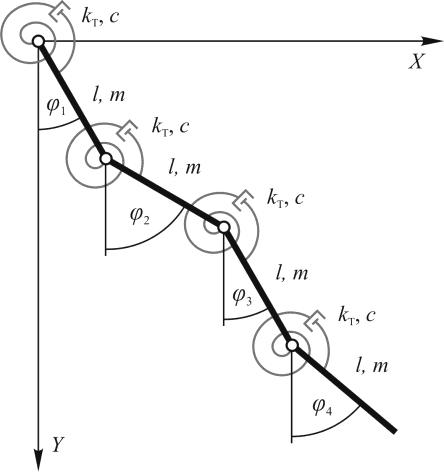
\includegraphics[width=0.42\textwidth]{11.nal_slike/Non-linear_dynamics_of_a_hanging_rope.jpg}
    \caption{Diskretni sistem}
\end{figure}

\begin{align}
    &\sum_{j=1}^{N}\; \underbrace{c(i,j)\,\cos(\varphi_i-\varphi_j)}_{A_{i,j}}\, \underbrace{\ddot\varphi_j}_{x_j} = \\\nonumber
    &\underbrace{-\sum_{j=1}^{N} \left[c(i,j)\,\dot\varphi_j^2\,\sin(\varphi_i-\varphi_j) \right] - \frac{g}{l}\,(N-i+1)\,\sin\varphi_i - \zeta\,c_{c}\,\dot\varphi_i}_{b_i}
\end{align}
kjer je $c(i,j) = N - \max(i,j) + 1$, $\varphi$ zasuk, $\dot\varphi$ kotna hitrost in $\ddot\varphi$ kotni pospešek v lokalnem polarnem koordinatnem sistemi i-tega delčka vrvi, $g$ velikost gravitacijskega pospešek in $N$ število diskretnih mas vrvi. Izpeljava teh enačb je povzeta po \cite{Taylor_Pendulum_2024} \cite{Assencio_double_pendulum} \cite{N_pendulum_1} \cite{N_pendulum_2}, pri čemer sem dodal model viskoznega dušenja zaradi stabilizacije simulacije, saj sicer sistem izkazuje kaotično naravo in nefizikalne oscilacije diskretnih mas (nihal). Drugače pa je na to temo ogromno literature in še več formulacij!

\section{Simulacija}

Za vse simulacije sem uporabljal brezdimenzijske enote, težnostni pospešek $g=1$ m/s$^2$, skupna masa $M=1$ kg in dolžina vrvi $L=1$ m. Diskretizacija je enakomerna: $l_i=L/N$ in $m_i = M/N$, kar je upoštevano že v sistemu gibalnih enačb.

Razmernik dušenja je karseda majhen, vendar vseeno dovolj velik, da izniči oscilacije $\zeta=7\cdot10^{-3}$. Pri manjših začetnih kotih, ko ne prihaja do efekta ``pokanja biča'', se sicer obnese tudi nedušen sistem, vendar, ko do tega pojava pride, tak sistem prične z oscilacijami členkov, kar je prikazano v prilogi \texttt{neduseno.mp4}. Z uvedbo razmernika dušenja simulacijo stabiliziramo, hkrati pa se doda nov fizikalen princip vanjo, saj `brez dušenja ni življenja'.

Kot začetne pogoje (ZP) sem predpostavil mirujočo vrv z različnimi legami. Ker je popis izveden v lokalnem polarnem koordinatnem sistemu za vsak členek, sem moral v njem tudi definirati lego vrvice. Nato sem rešil sistem gibalnih enačb in izvedel časovno integracijo z metodo \textit{Runge-Kutta 4.reda} s časovnim korakom $\Delta t = 0.01$ do časa $T$, ki je definiran kot čas treh (teoretičnih) nihajev matematičnega nihala $T= 3\, \frac{2\,\pi}{\omega_{0d}} = 18.9$~s.

Kjer so prikazan le končna stanja simulacij, so animacije shranjene kot priloge v obliki \textit{mp4} datotek. Energije sem računal po njihovih osnovnih definicijah.

\subsection{Začetni pogoj ravne mirujoče vrvice pod kotom $\varphi_0$}

Začetne pogoje za ravno vrvico je enostavno doseči; definiram željeni kot v radianih za vsak členek. Na spodnji sliki je prikazano končno stanje po 3 teoretičnih nihajih. Že takoj opazim, da je resnične frekvenca nihanja vrvi malenkost večja od matematičnega nihala, saj vrv naredi v danem času več kot 3 nihaje.

Pri 45$^\circ$ je nihanje vrvi še načeloma podobno mat. nihalu, dodatno se le vrv upogiba. Pri 90$^\circ$ pa je opazen ``udarec biča'' v prvem nihaju, kar povzroča največje težave pri časovni integraciji in odločilno vpliva na način nihanja. Pot zadnje točke se očitno razlikuje od 45$^\circ$. Iz primerjav je razvidno, da ima integrator težave z ohranjanjem energij, kar se z večanjem $\varphi_0$ le povečuje.

Preizkusil sem še ``prosti padec'' vrvi, ko je začetni kot enak 180$^\circ$. Zanimivo je, da, čeprav sem pričakoval nihanje le v y-smeri, prihaja do rotacije vrvi. Taka rešitev ni fizikalna, saj bi v tem primeru moral upoštevati tudi torzijo v vrvi, preseneča me pa, da, kot je razvidno iz primerjav med poz. in neg. začetnim kotom, le ta vpliva na smer rotacije vrvi, potek energij je namer povsem enak, koordinate pa le zrcaljene preko y-osi. Mogoče je to posledica numerične napake pri integraciji, vendar je natanko tako ob vsaki ponovitvi, kar mi vzbuja sum, da je za to ``kriva'' izpeljava gibalnih enačb.

\begin{figure}[H]
    \centering
    \begin{subfigure}{0.49\textwidth}
        \centering
        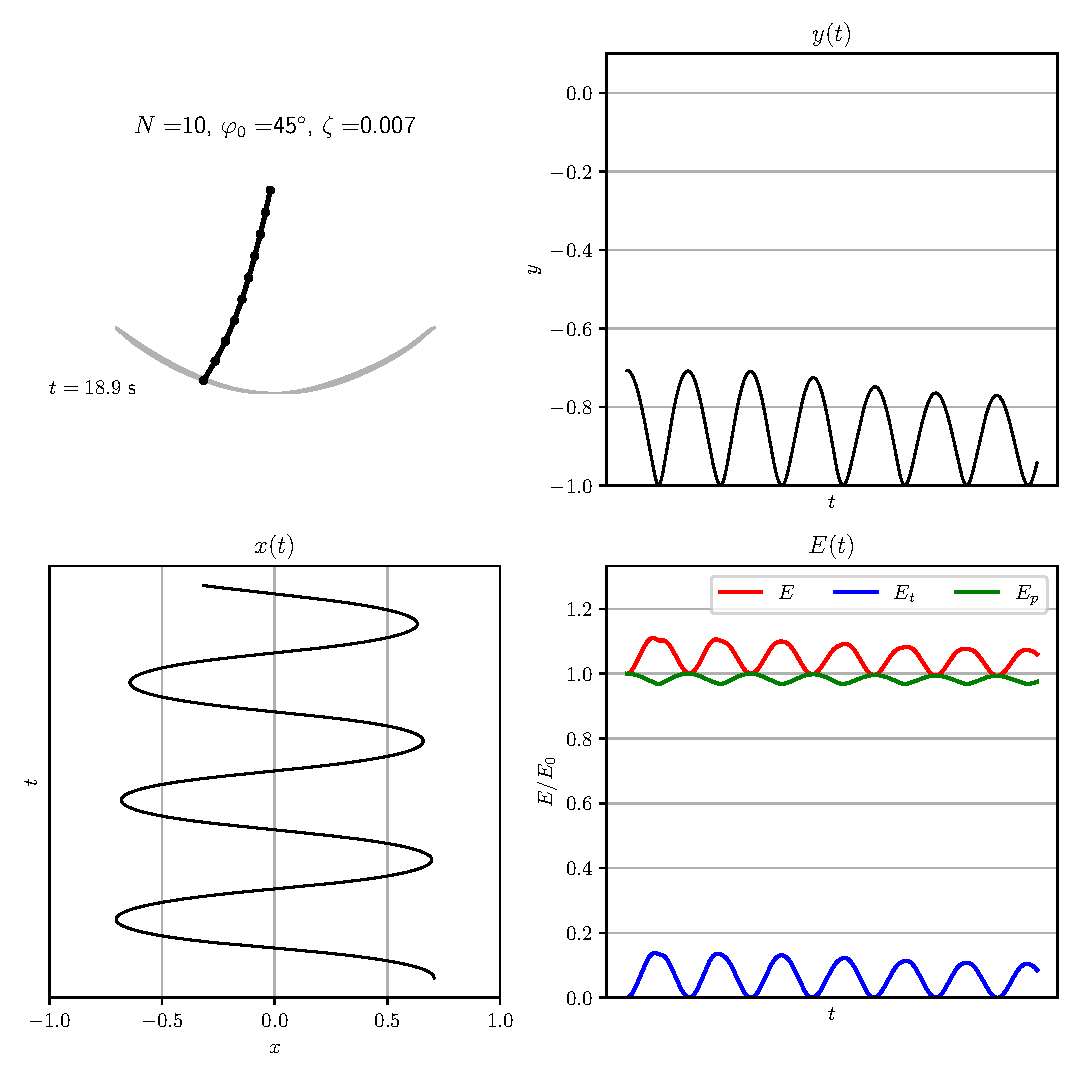
\includegraphics[width=\linewidth]{11.nal_slike/pendulum_N10_phi45.pdf}
        \caption{\texttt{pendulum\_N10\_phi45.pdf}}
    \end{subfigure}
    \begin{subfigure}{0.49\textwidth}
        \centering
        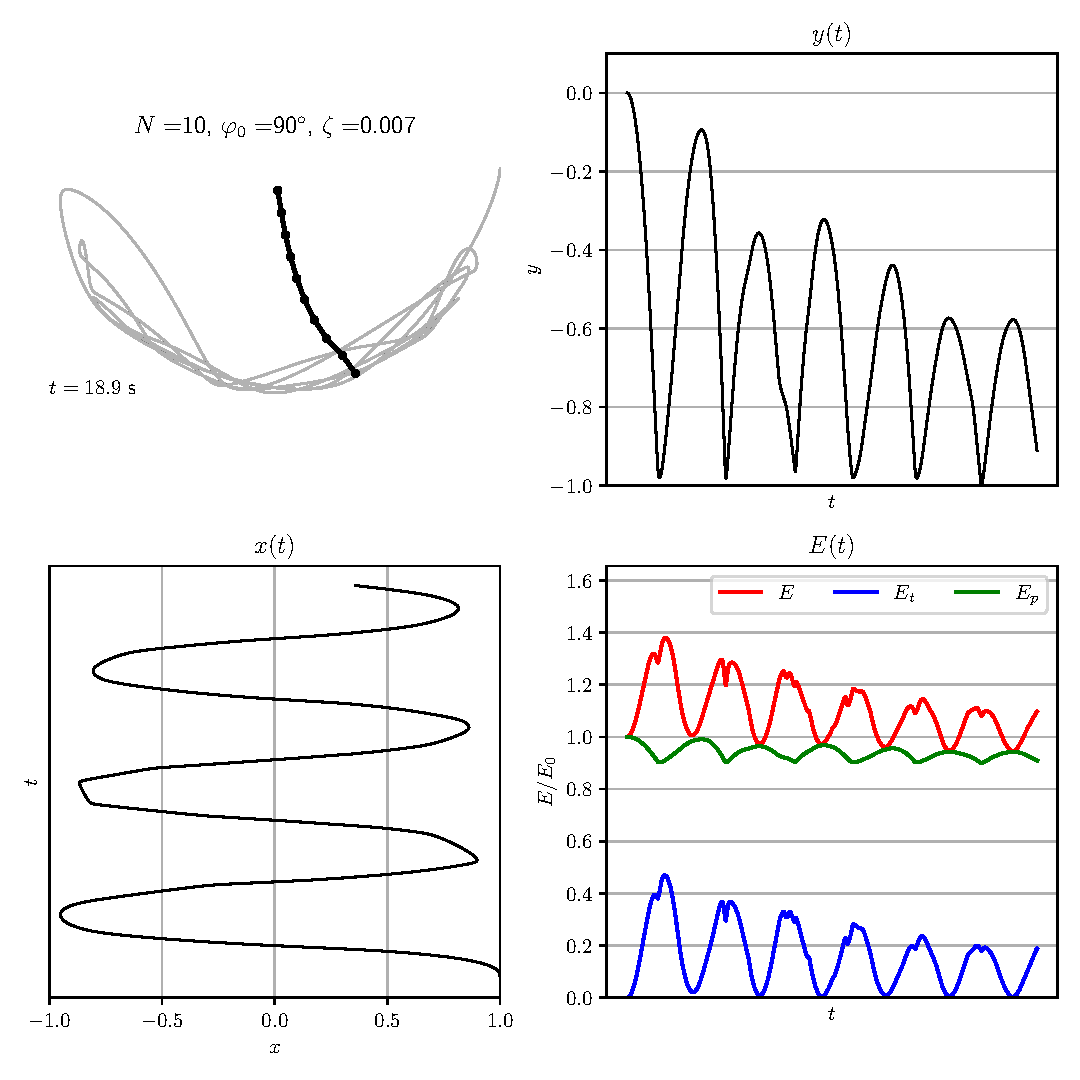
\includegraphics[width=\linewidth]{11.nal_slike/pendulum_N10_phi90.pdf}
        \caption{\texttt{pendulum\_N10\_phi90.pdf}}
    \end{subfigure}
    \begin{subfigure}{0.49\textwidth}
        \centering
        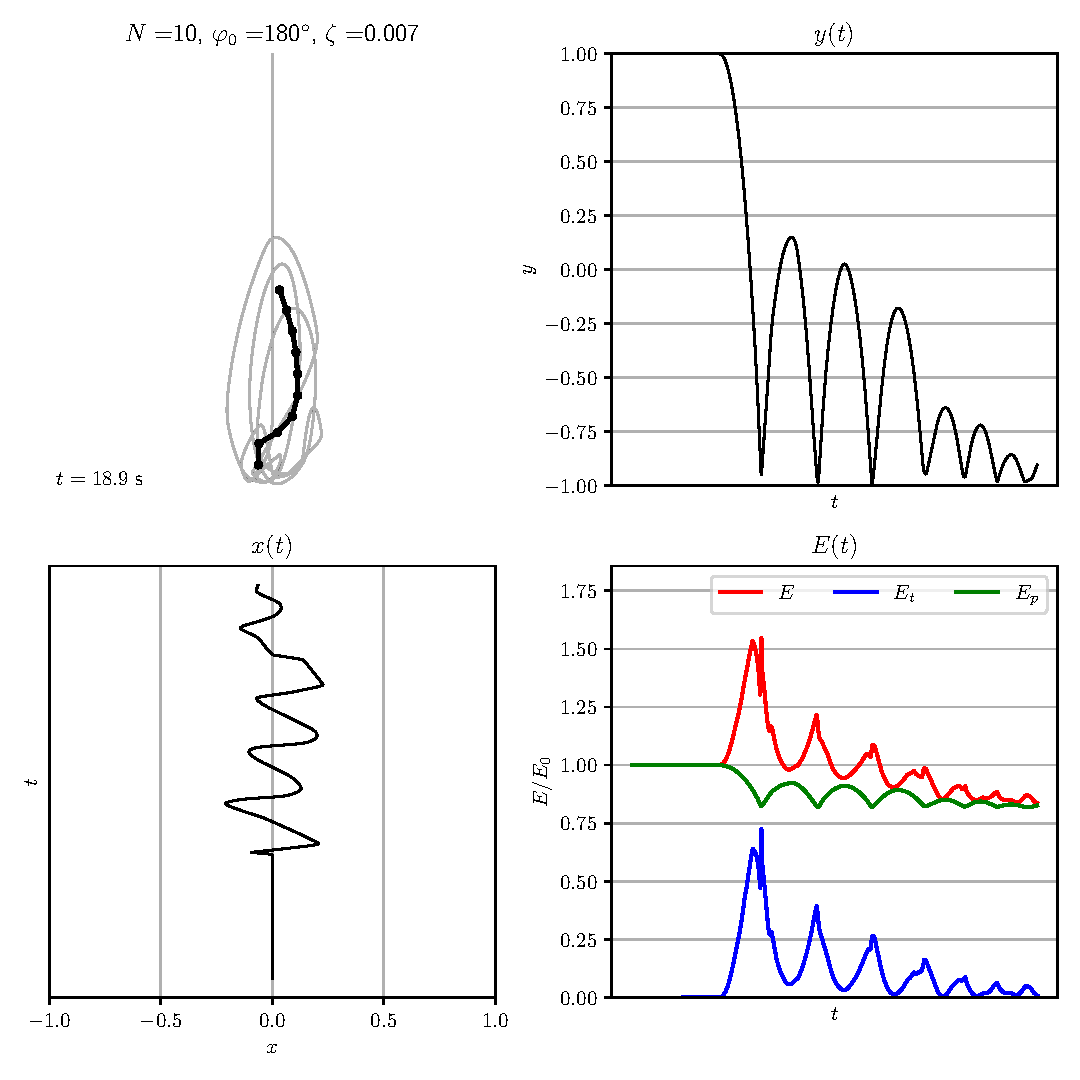
\includegraphics[width=\linewidth]{11.nal_slike/pendulum_N10_phi180.pdf}
        \caption{\texttt{pendulum\_N10\_phi180.pdf}}
    \end{subfigure}
    \caption{Končna stanja simulacij iz animacij v prilogi}
\end{figure}

\begin{figure}[H]
    \centering
    \begin{subfigure}{0.45\textwidth}
        \centering
        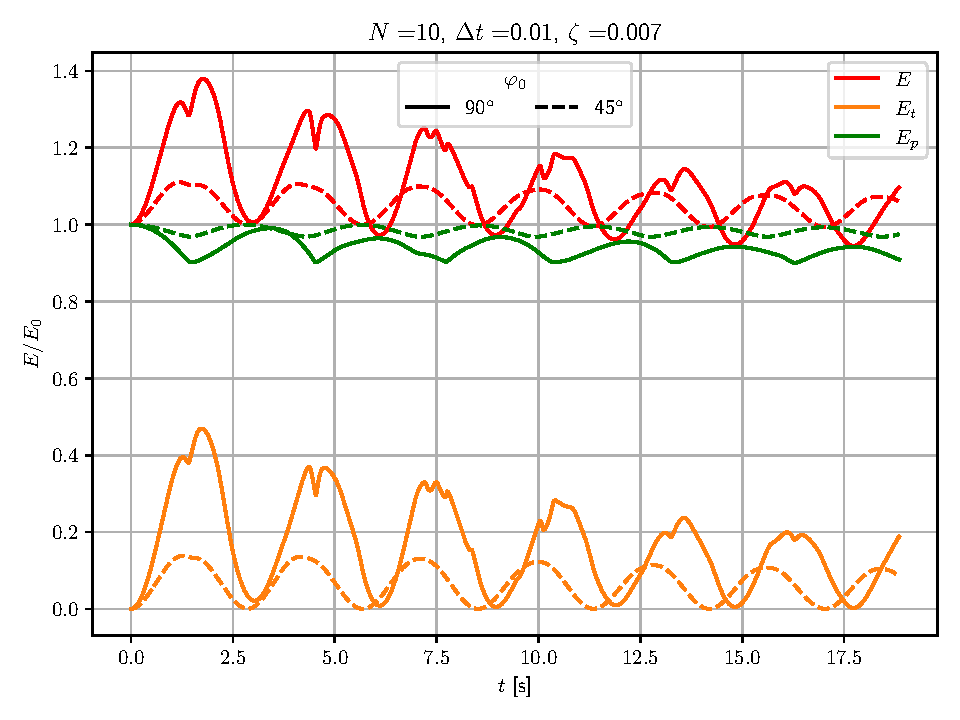
\includegraphics[width=\linewidth]{11.nal_slike/energije_N10_phi90-45.pdf}
        \caption{\texttt{primerjava\_phi90\_45.pdf}}
    \end{subfigure}
    \begin{subfigure}{0.45\textwidth}
        \centering
        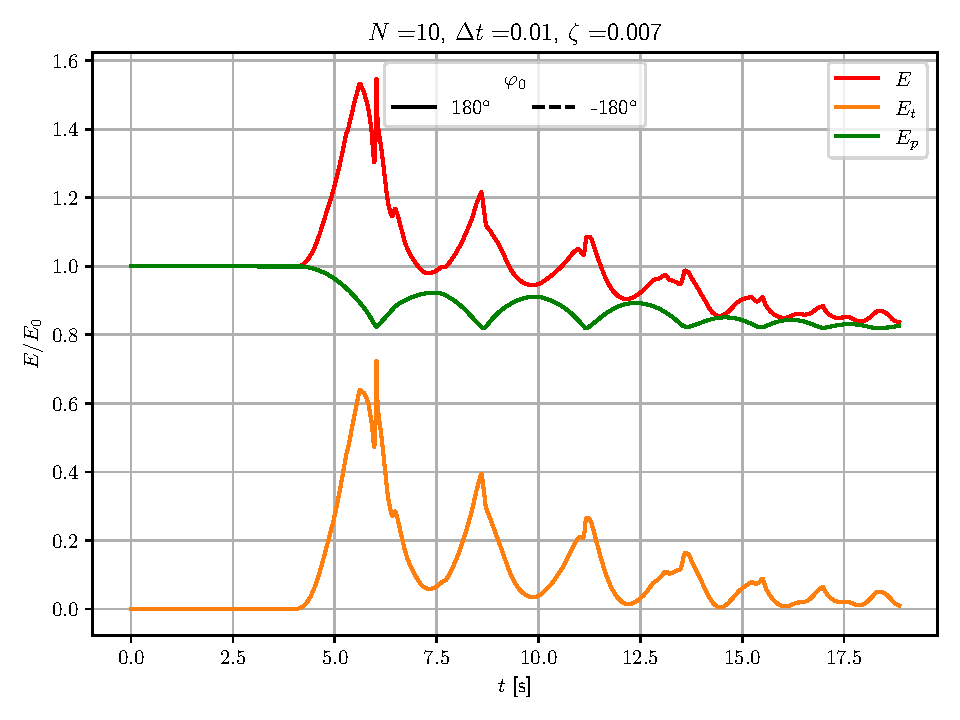
\includegraphics[width=\linewidth]{11.nal_slike/energije_N10_phi180--180.pdf}
        \caption{\texttt{primerjava\_phi180\_-180.pdf}}
    \end{subfigure}
    \caption{Primerjava potekov energij za različne začetne pogoje iz animacij v prilogi}
\end{figure}

\subsection{Začetni pogoj vrvi v obliki parabole}

Ker je ZP ravne vrvi precej nerealen, uporabim približno začetno obliko vrvi pod lastno težo - parabolo. Opazim, da taka oblika le še poveča ``pokanje biča'', saj je ta opazen že pri 45$^\circ$ v sicer milejši obliki. Nihanje vrvi se tako močno spremeni, saj se v njen pojavi tudi prečno nihanje, kot je opazno pri 90$^\circ$ iz prejšnjega poglavja. Za popis prečnih nihajev bi potreboval gostejšo diskretizacijo, kar pa močno poveča računski čas.

Glede na ZP iz prejšnjega poglavja, to poleg večje amplitude poveča tudi energijska nihanja.

\begin{figure}[H]
    \centering
    \begin{subfigure}{0.49\textwidth}
        \centering
        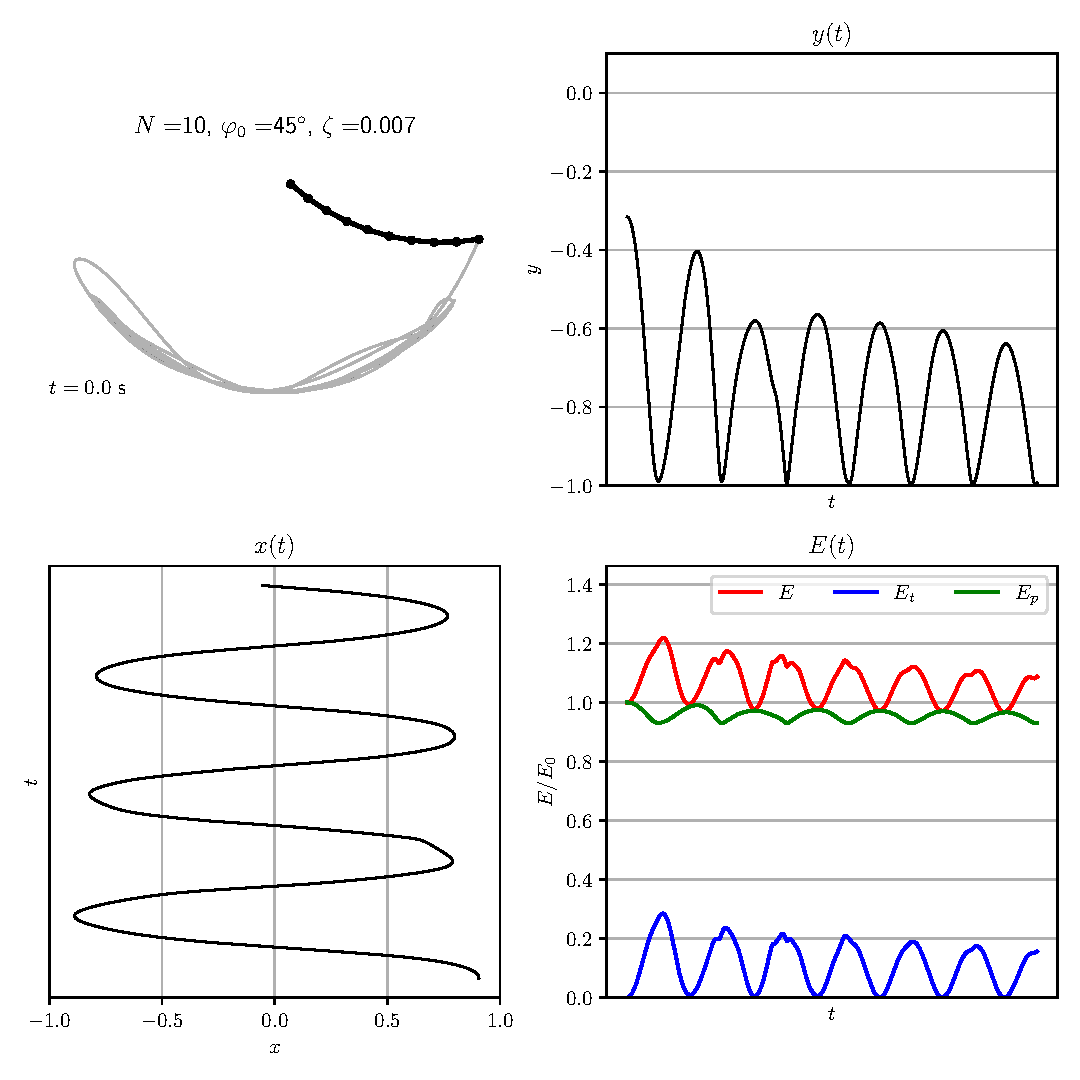
\includegraphics[width=\linewidth]{11.nal_slike/pendulum_N10_phi45_parabola.pdf}
        \caption{\texttt{pendulum\_N10\_phi45\_parabola.pdf}}
    \end{subfigure}
    \begin{subfigure}{0.49\textwidth}
        \centering
        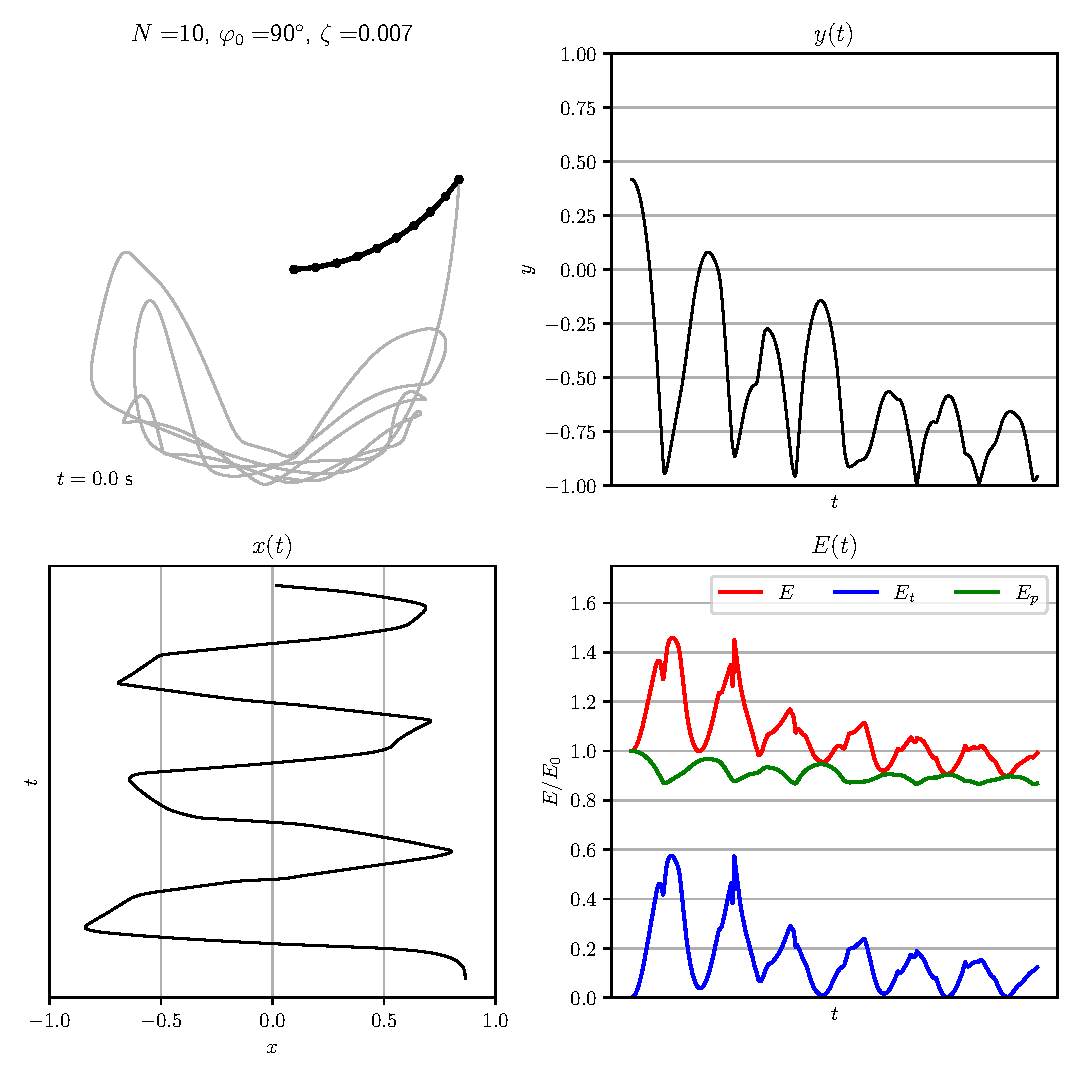
\includegraphics[width=\linewidth]{11.nal_slike/pendulum_N10_phi90_parabola.pdf}
        \caption{\texttt{pendulum\_N10\_phi90\_parabola.pdf}}
    \end{subfigure}
    \caption{Končna stanja simulacij iz animacij v prilogi, vrv je prikazana v ZP.}
\end{figure}

\begin{figure}[H]
    \centering
    \begin{subfigure}{0.45\textwidth}
        \centering
        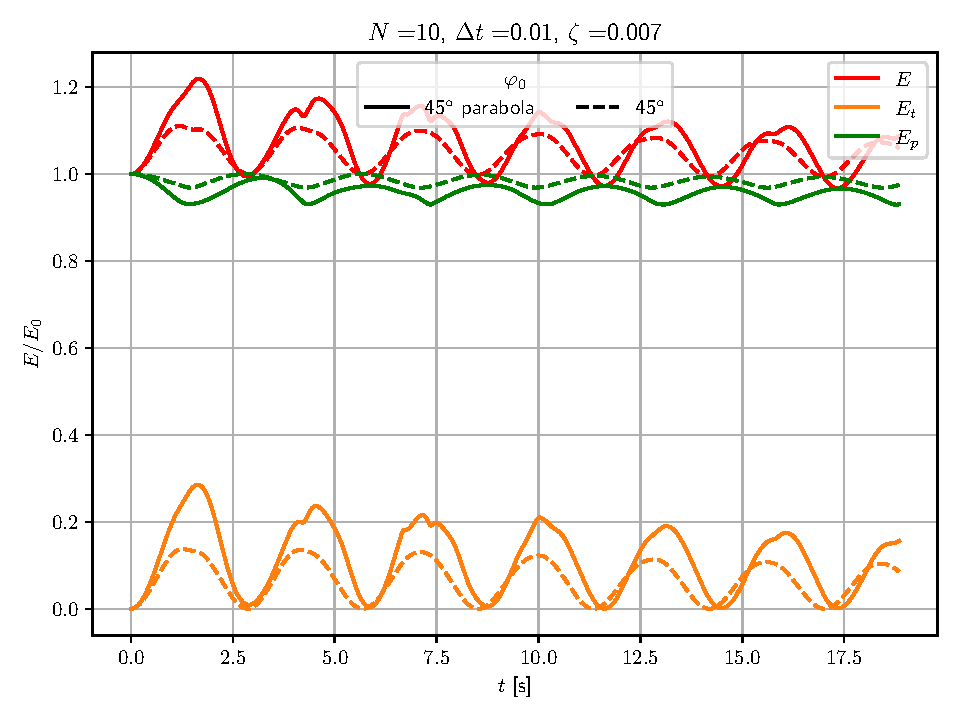
\includegraphics[width=\linewidth]{11.nal_slike/energije_N10_phi45-45_parabola.pdf}
        \caption{\texttt{primerjava\_phi45\_45\_parabola.pdf}}
    \end{subfigure}
    \begin{subfigure}{0.45\textwidth}
        \centering
        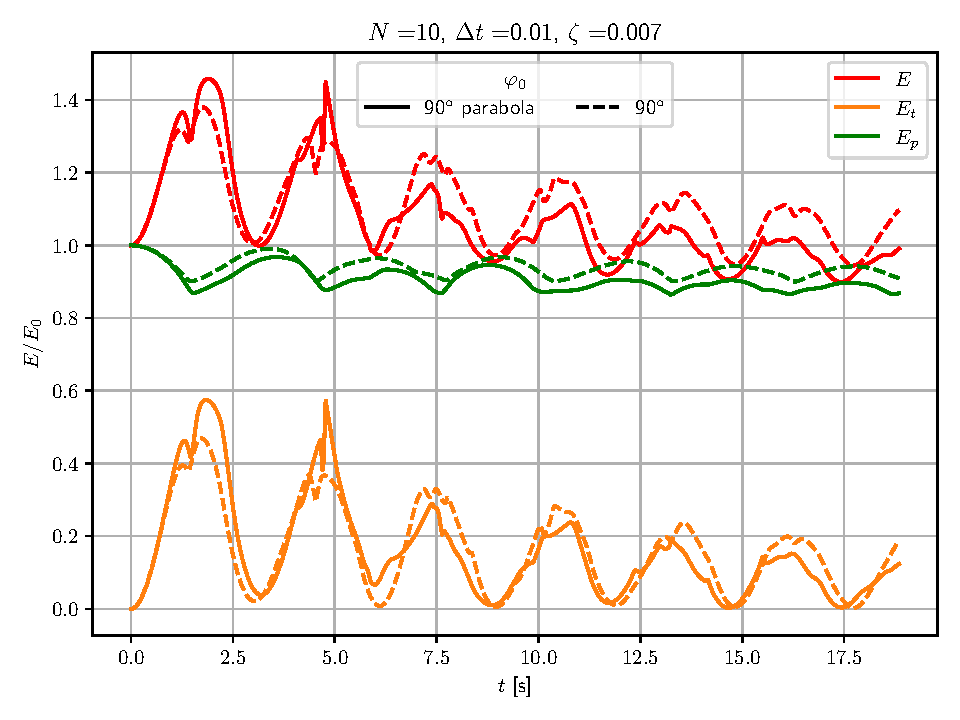
\includegraphics[width=\linewidth]{11.nal_slike/energije_N10_phi90-90_parabola.pdf}
        \caption{\texttt{primerjava\_phi90\_90\_parabola.pdf}}
    \end{subfigure}
    \caption{Primerjava potekov energij za animacije v prilogi med ravnim in paraboličnim ZP}
\end{figure}

\subsection{Začetni pogoj valovanja vrvi}

Preizkusil sem še bolj eksotičen ZP v obliki potujočega vala na vrvi, ki pa seveda ne potuje naprej po vrvi. Val je deloval kot dušilec nihanja v y-smeri, saj vzpodbudi nastanek prečnih valov na vrvi, ki bi bili bolje vidni ob še gostejši diskretizaciji. Prečnih nihanj pri ZP ravne vrvi do 45$^\circ$ ni zaznati! Tudi če sem obrnil smer parabole, torej da je zakrivljena navzdol, je moč opaziti podobne lastnosti (\texttt{pendulum\_N20\_phi90\_parabola\_obratno.mp4}).
\begin{figure}[H]
    \centering
    \begin{subfigure}{0.49\textwidth}
        \centering
        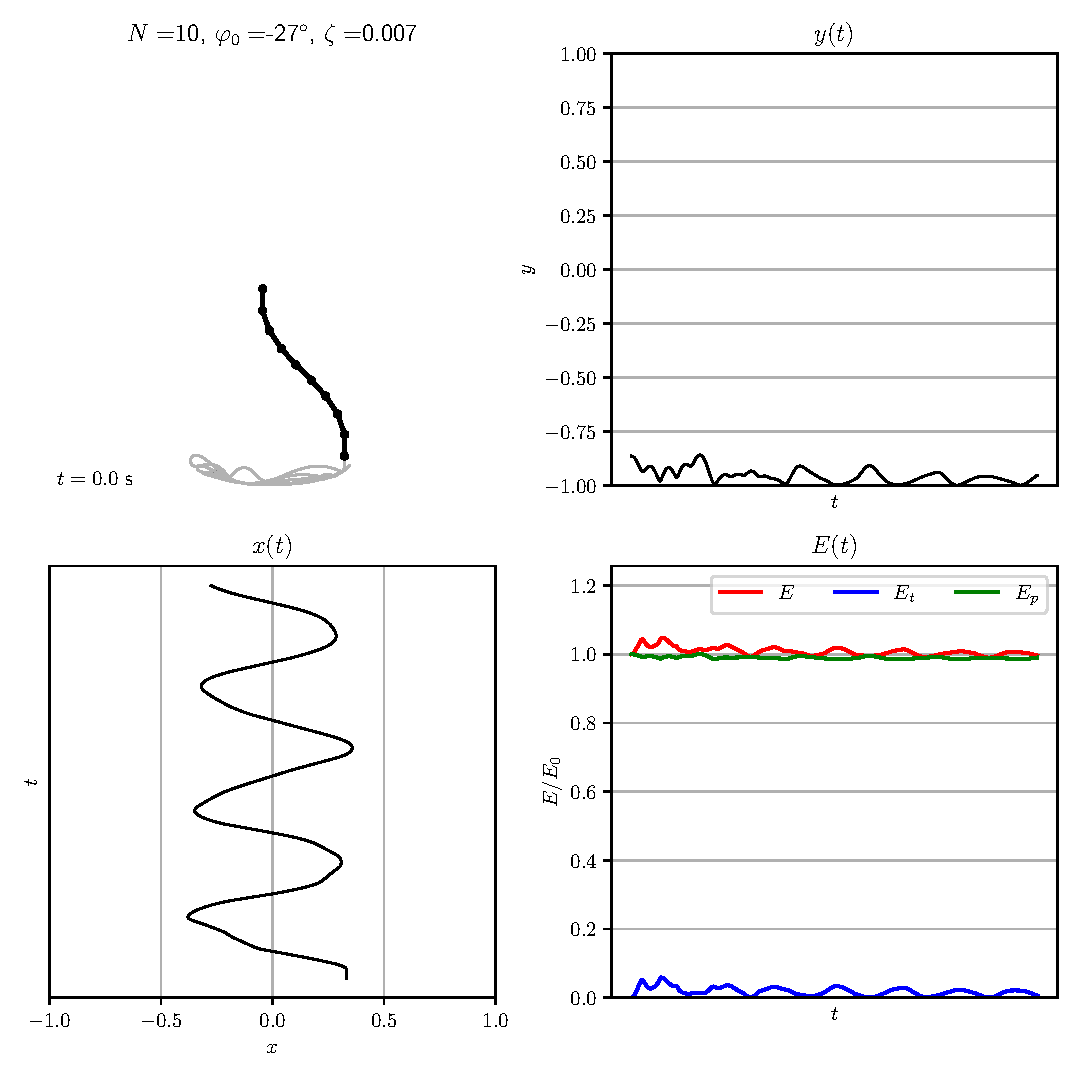
\includegraphics[width=\linewidth]{11.nal_slike/pendulum_N10_val.pdf}
        \caption{\texttt{pendulum\_N20\_val.pdf}}
    \end{subfigure}
    \begin{subfigure}{0.49\textwidth}
        \centering
        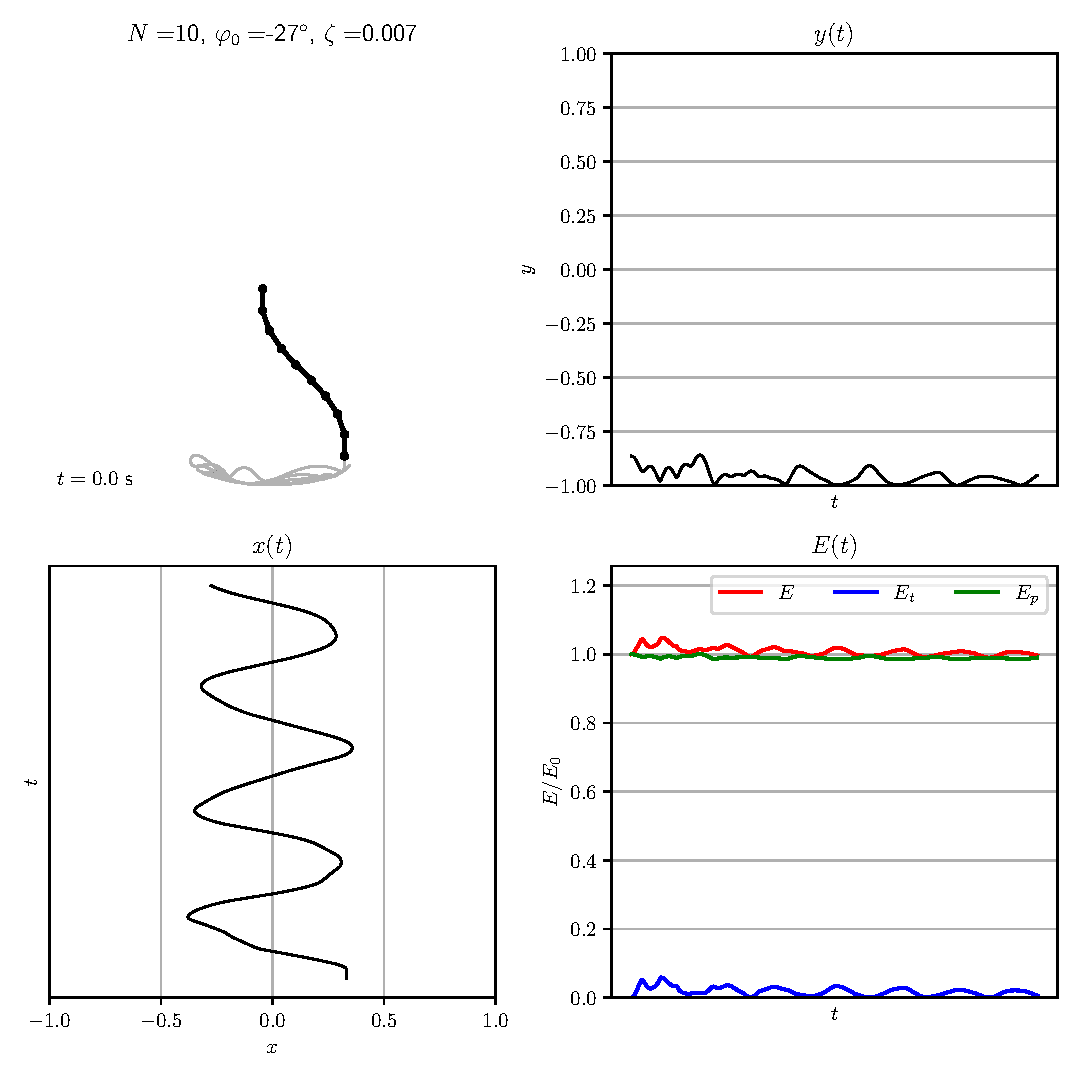
\includegraphics[width=\linewidth]{11.nal_slike/pendulum_N10_val.pdf}
        \caption{\texttt{pendulum\_N20\_parabola\_obratno.pdf}}
    \end{subfigure}
    \caption{Končno stanje simulacije iz animacij v prilogi, vrv je prikazana v ZP.}
\end{figure}

\section{Analiza dinamike vrvi}

Uporabil sem enake parametre simulacije kot v prejšnjem poglavju s to razliko, da sem simuliral čas 50 nihajev mat. nihala (314 s). V tem primeru sem spreminjal ZP ravne vrvi (naklon) in diskretizacijo. Predvsem sem se osredotočil na določitev lastnih frekvenc nihajoče vrvi, za prehod v frekvenčno domeno sem uporabil algoritem FFT v \textit{numpy} in okensko funkcijo \textit{Hann} za zmanjšanje frekvenčnega puščanja. Izkazalo se bo, da bi bilo bolje, če bi uporabil še daljši čas simulacije, kar bi povečalo frekvenčno ločljivost, saj se dodajanje ničel (zero-padding) na koordinatah ni obneslo dobro.

\subsection{Odvisnost od diskretizacije}

Poglejmo, kako diskretizacija vpliva na 1. lastno frekvenco vrvi. Če $N=1$ je to kar frekvenca matematičnega nihala, z povečevanjem pa narašča in konvergira k 1. lastni frekvenci prosto nihajoče se neraztegljive vrvi brez togosti.

Za aproksimacijo sem uporabil sigmoidno funkcijo, vendar se izkaže, da to ni najbolje, saj je zadnja vrednost vseeno nad $f(\infty)$. Moč je opaziti, da frekvence zavzemajo diskretne nivoje; temu je kriva frekvenčna ločljivost, kar je omenjeno že na začetku tega poglavja.

\begin{figure}[H]
    \centering
    \begin{subfigure}{0.49\textwidth}
        \centering
        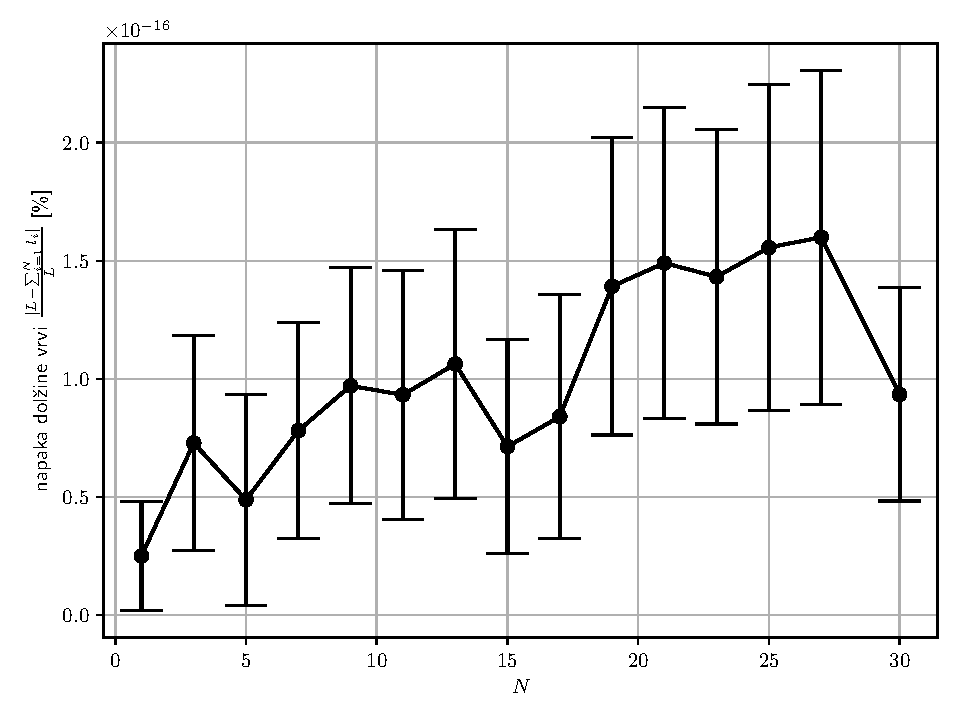
\includegraphics[width=\linewidth]{11.nal_slike/napaka_L_od_N.pdf}
        \caption{Povprečna napaka izračunov dolžine vrvi}
    \end{subfigure}
    \begin{subfigure}{0.49\textwidth}
        \centering
        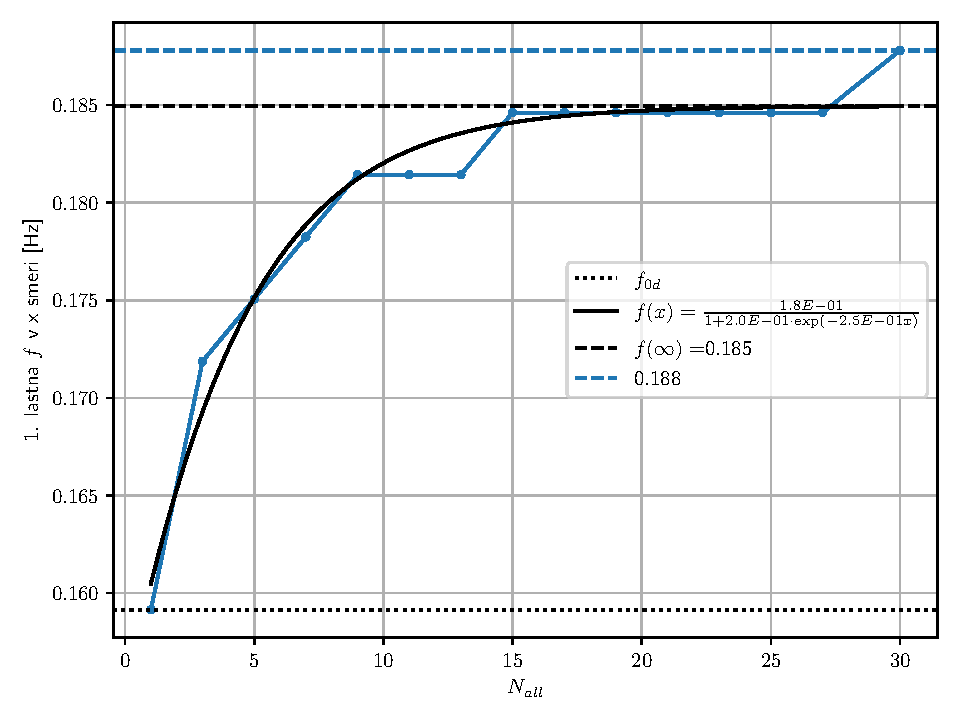
\includegraphics[width=\linewidth]{11.nal_slike/konv_N.pdf}
        \caption{Konvergenca 1. lastne frekvence}
    \end{subfigure}
    \caption{Simulacija z različnimi gostotami diskretizacij vrvi $N$}
\end{figure}

Sicer pa pri sledečih amplitudnih in faznih spektrih frekvenčne ločljivosti sploh ni opaziti. Iz njih lahko izluščimo lastne frekvence vrvi kot vrh pri amplitudnem spektru, prav tako pa se takrat obrne faza nihanja, kar vidimo v amplitudnem spektru. Zaradi šuma pri FFT in dejstva, da se v anti-resonanci tudi obrne faza, je določevanje iz faznega spektra težje, zato sem vrhove določeval na amplitudi s \textit{scipy.optimize.find\_peaks}. Pričakovano ima nihanje v y-smeri in nihanje energij 2x večjo lastno frekvenco od x-smeri.

Več vrhov je prisotnih zaradi dušenja, pri matematičnem nihalu je vrh le pri $\omega_{0d}$, preostali so posledica puščanja, kar me preseneča, zakaj v tem primeru okenska funkcija odpove. Za tak preproste primere, z malo $N$, ko ne pride do ``pokanja biča'', sicer dušenje ni potrebno, vendar zaradi konsistentnosti s preostalimi grafi simuliram vse dušeno.

Matematičnemu nihalu se lahko približam le brez dušenja in z majhnim začetnim kotom, kar je glavna predpostavka linearizacije gibalne enačbe. Tak sistem je najbolje simulirati le z eno maso, saj sem sistem gibalnih enačb izpeljal za enakomerno diskretizacijo s konstantno porazdelitvijo mase.

\begin{figure}[H]
    \centering
    \begin{subfigure}{0.45\textwidth}
        \centering
        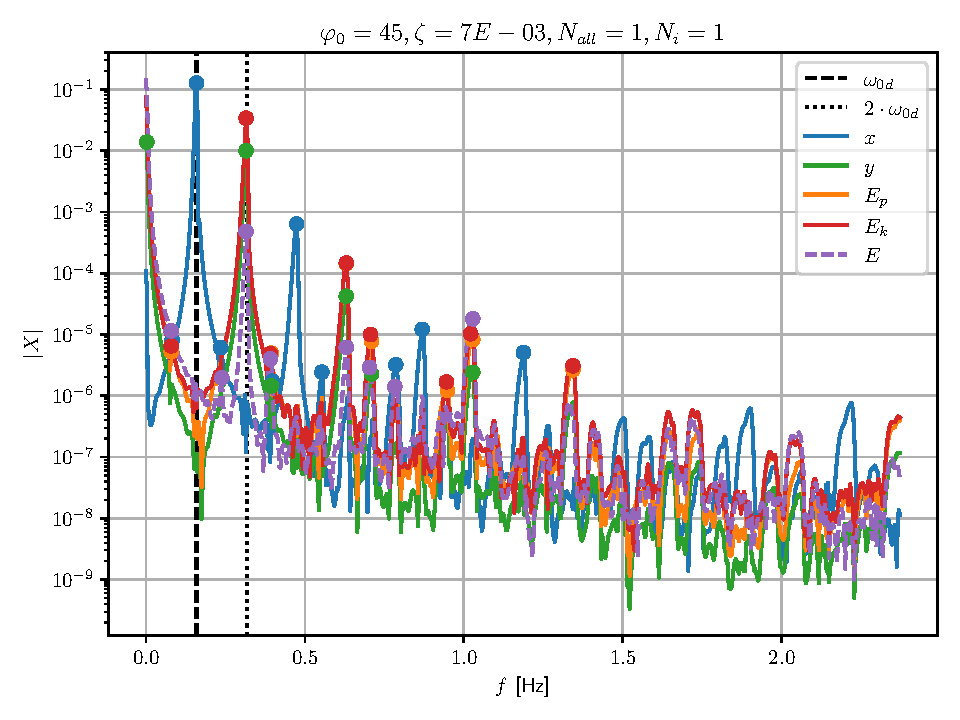
\includegraphics[width=\linewidth]{11.nal_slike/dinamika/fft_lastne_Ni1_phi45_N1.pdf}
        \caption{Amplitudni spekter}
    \end{subfigure}
    \begin{subfigure}{0.45\textwidth}
        \centering
        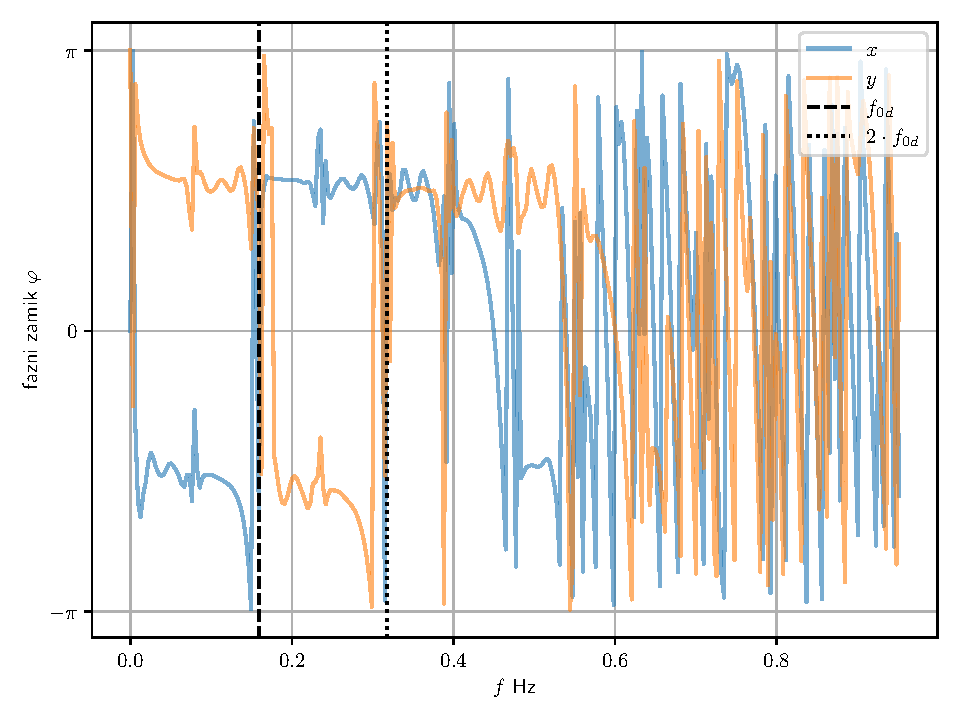
\includegraphics[width=\linewidth]{11.nal_slike/dinamika/fazni zamik_N1_phi45_N1.pdf}
        \caption{Fazni spekter}
    \end{subfigure}
    \caption{FFT pri diskretizaciji $N=1$ in ZP ravna vrv $\varphi_0=45^\circ$}
\end{figure}

\begin{figure}[H]
    \centering
    \begin{subfigure}{0.45\textwidth}
        \centering
        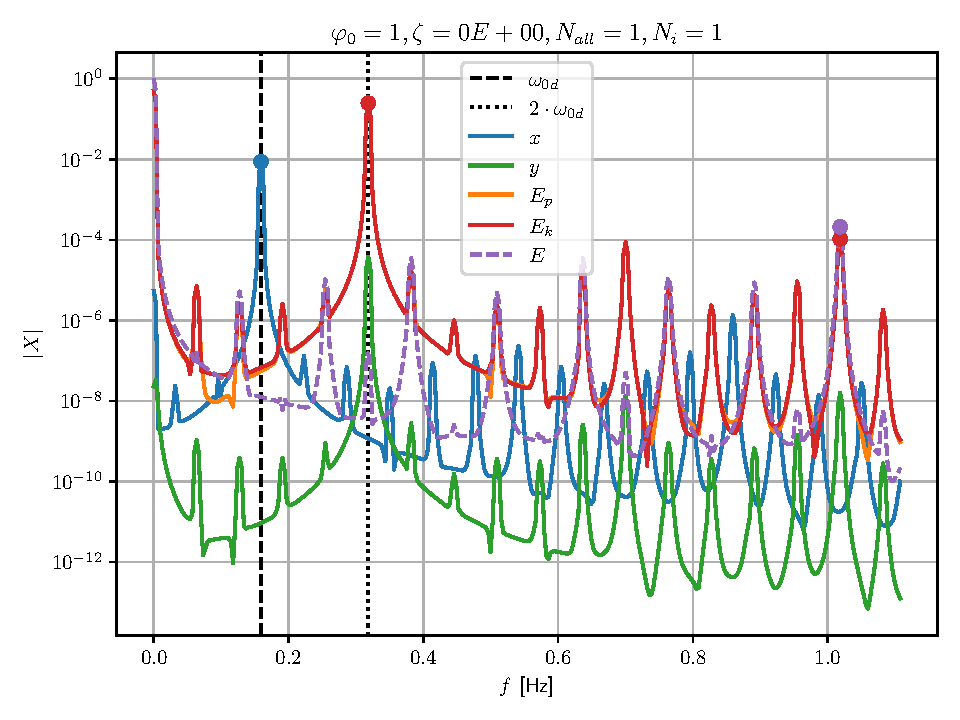
\includegraphics[width=\linewidth]{11.nal_slike/dinamika/fft_lastne_Ni1_phi1_N1_nedus.pdf}
        \caption{Amplitudni spekter}
    \end{subfigure}
    \begin{subfigure}{0.45\textwidth}
        \centering
        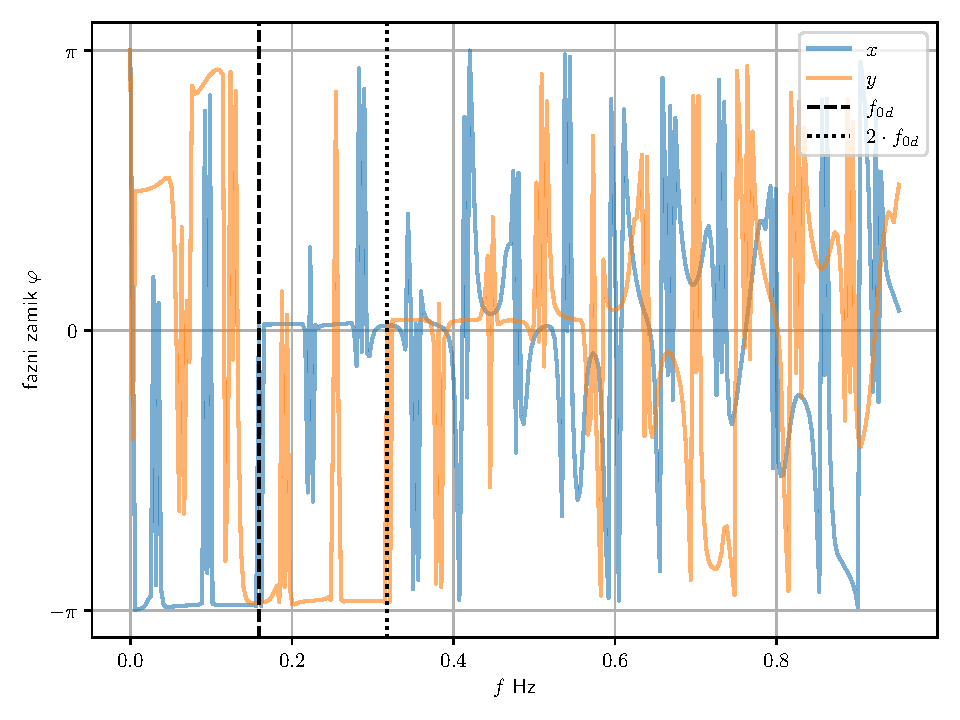
\includegraphics[width=\linewidth]{11.nal_slike/dinamika/fazni zamik_N1_phi1_N1_nedus.pdf}
        \caption{Fazni spekter}
    \end{subfigure}
    \caption{FFT pri diskretizaciji $N=1$ in ZP ravna vrv $\varphi_0=1^\circ$, matematično nihalo}
\end{figure}

Ako dodamo dve nihajoči masi ($N=2$), se težava določanja vrhov le še poveča. Opazno je lastna frekvenca že malo večja od matematičnega nihala! Bolje je določati na zadnji masi, saj so tam amplitude večje in lažje določim večje število vrhov (nekako do 3. lastne frekvence).
Enako in še bolj očitno velja za večje $N$, le da je pri porazdelitvi 1. lastne frekvence po dolžini vrvi ponovno nagajala frekvenčna ločljivost, fazni spekter pa je vedno težje berljiv zaradi pojavov manjših vrhov, ki povzročijo fazne zamike.

\begin{figure}[H]
    \centering
    \begin{minipage}{0.45\textwidth}
        \centering
        \begin{subfigure}{\linewidth}
            \centering
            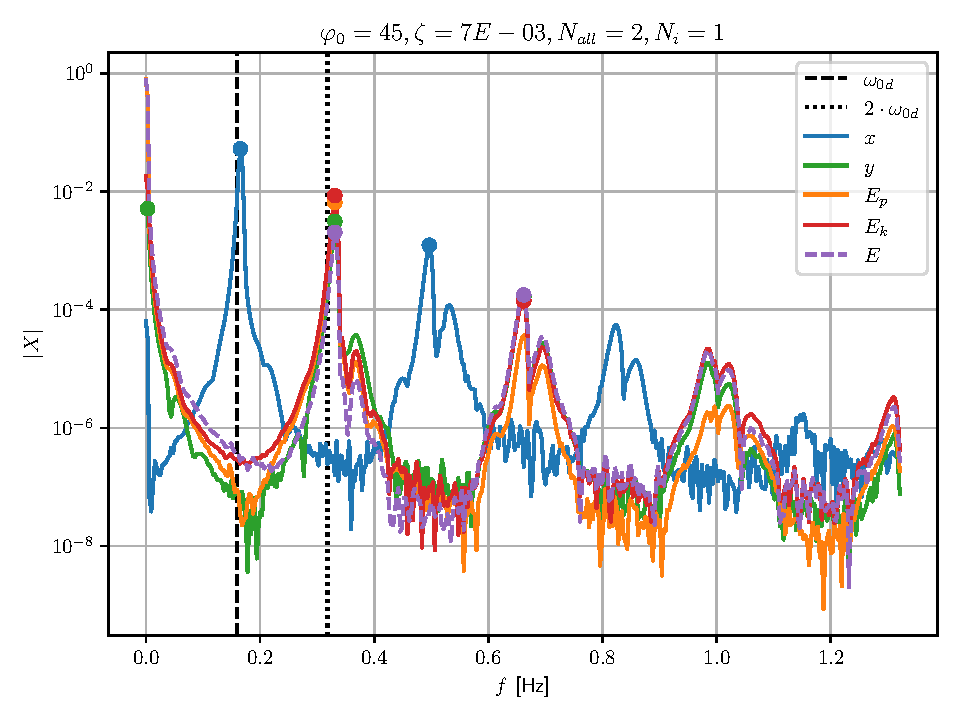
\includegraphics[width=\linewidth]{11.nal_slike/dinamika/fft_lastne_Ni1_phi45_N2.pdf}
            \caption{Amplitudni spekter v masi 1}
        \end{subfigure}
        \begin{subfigure}{\linewidth}
            \centering
            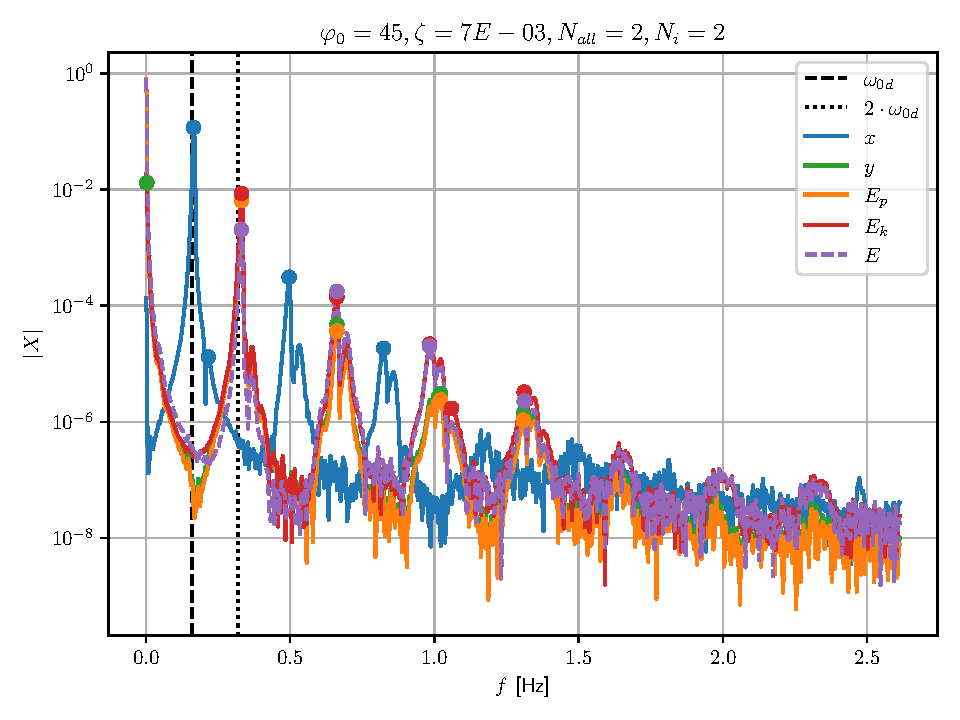
\includegraphics[width=\linewidth]{11.nal_slike/dinamika/fft_lastne_Ni2_phi45_N2.pdf}
            \caption{Amplitudni spekter v masi 2}
        \end{subfigure}
    \end{minipage}
    \begin{minipage}{0.45\textwidth}
        \centering
        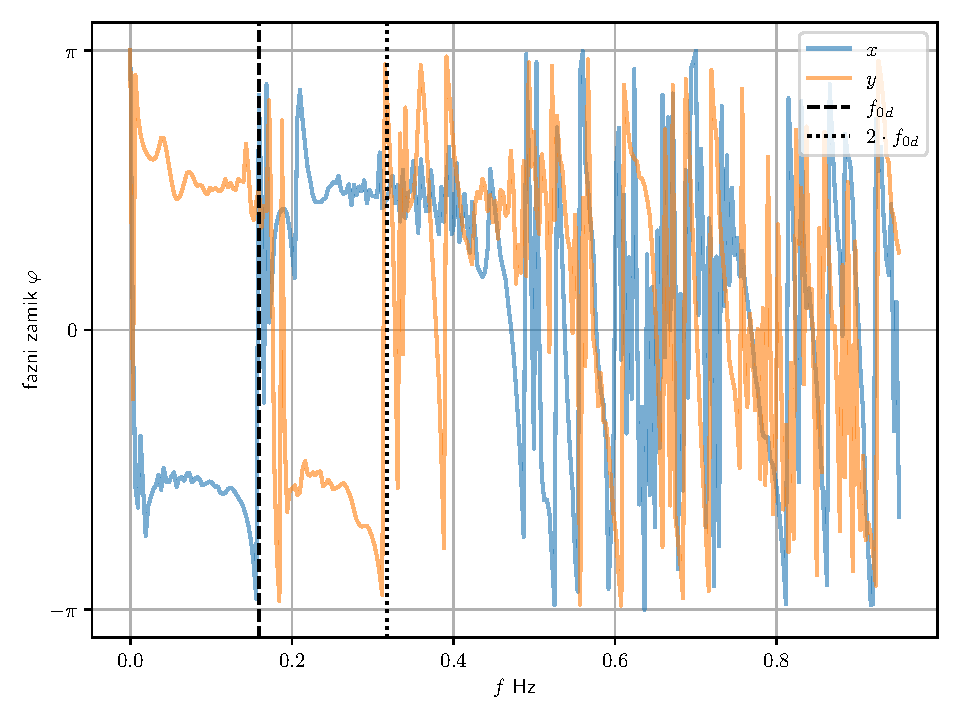
\includegraphics[width=\linewidth]{11.nal_slike/dinamika/fazni zamik_N2_phi45_N2.pdf}
        \caption{Fazni spekter v masi 2}
    \end{minipage}
    \caption{FFT pri diskretizaciji $N=2$ in ZP ravna vrv $\varphi_0=45^\circ$}
\end{figure}

\begin{figure}[H]
    \centering
    \begin{minipage}{0.45\textwidth}
        \centering
        \begin{subfigure}{\linewidth}
            \centering
            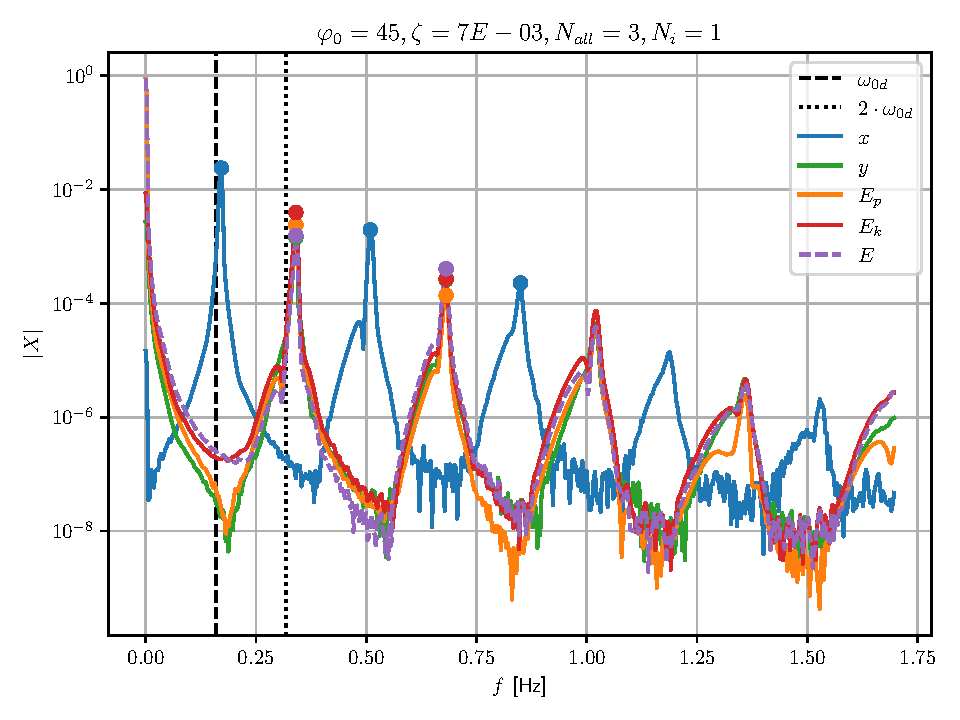
\includegraphics[width=\linewidth]{11.nal_slike/dinamika/fft_lastne_Ni1_phi45_N3.pdf}
            \caption{Amplitudni spekter v prvi masi}
        \end{subfigure}
        \begin{subfigure}{\linewidth}
            \centering
            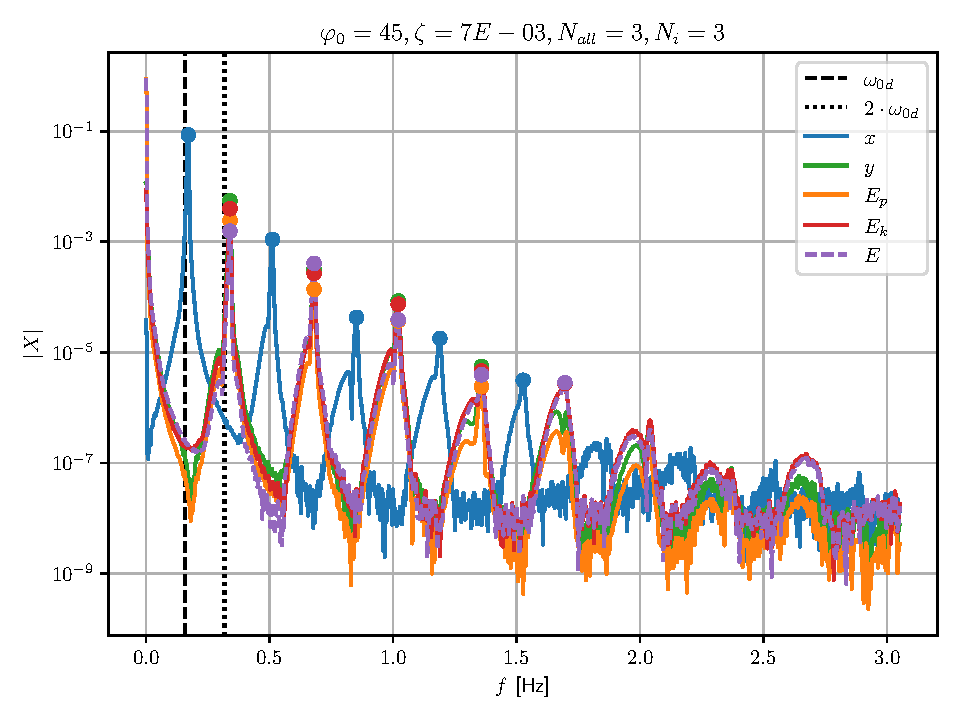
\includegraphics[width=\linewidth]{11.nal_slike/dinamika/fft_lastne_Ni3_phi45_N3.pdf}
            \caption{Amplitudni spekter v zadnji masi}
        \end{subfigure}
    \end{minipage}
    \begin{minipage}{0.45\textwidth}
        \centering
        \begin{subfigure}{\linewidth}
            \centering
            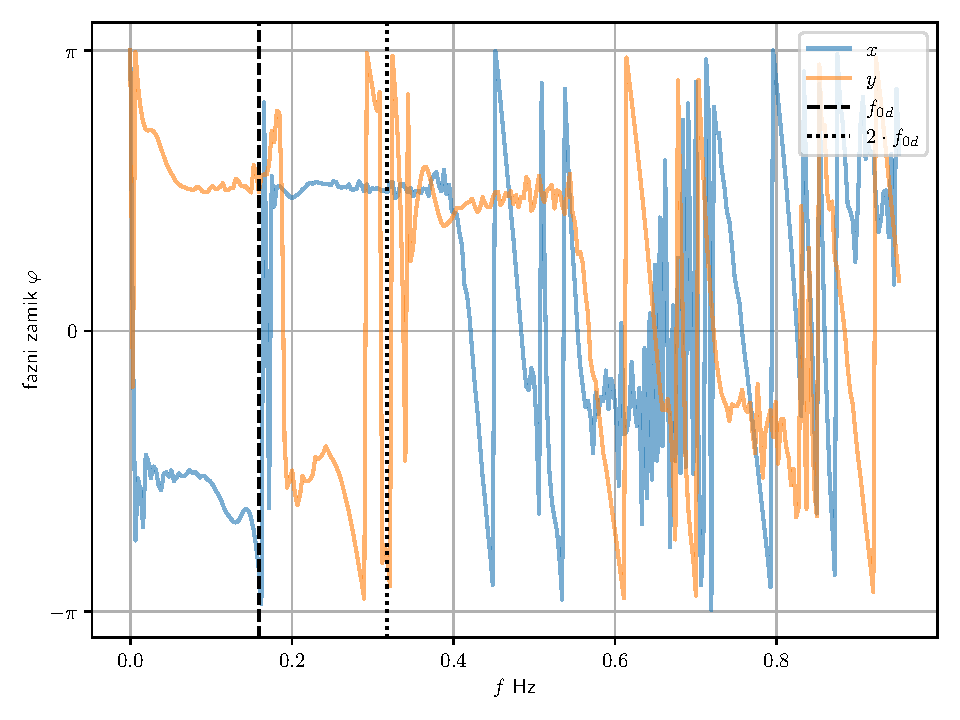
\includegraphics[width=\linewidth]{11.nal_slike/dinamika/fazni zamik_N3_phi45_N3.pdf}
            \caption{Fazni spekter v zadnji masi}
        \end{subfigure}
        \begin{subfigure}{\linewidth}
            \centering
            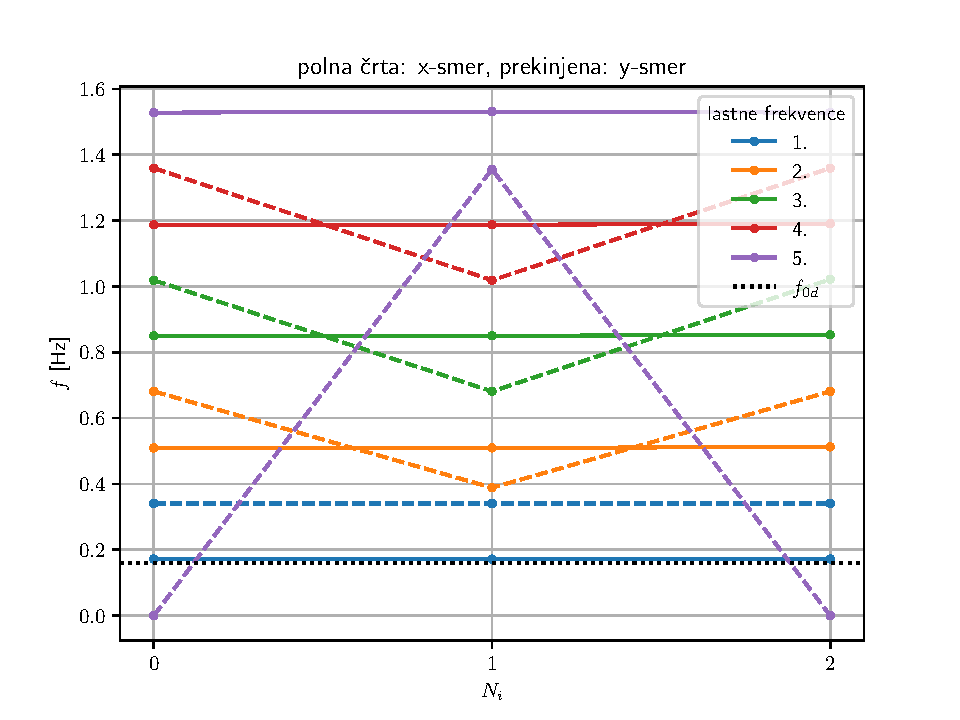
\includegraphics[width=\linewidth]{11.nal_slike/dinamika/vse_lastne_od_lege_phi45_N3.pdf}
            \caption{Lastne frekvence}
        \end{subfigure}
    \end{minipage}
    \caption{FFT pri diskretizaciji $N=3$ in ZP ravna vrv $\varphi_0=45^\circ$}
\end{figure}

\begin{figure}[H]
    \centering
    \begin{minipage}{0.45\textwidth}
        \centering
        \begin{subfigure}{\linewidth}
            \centering
            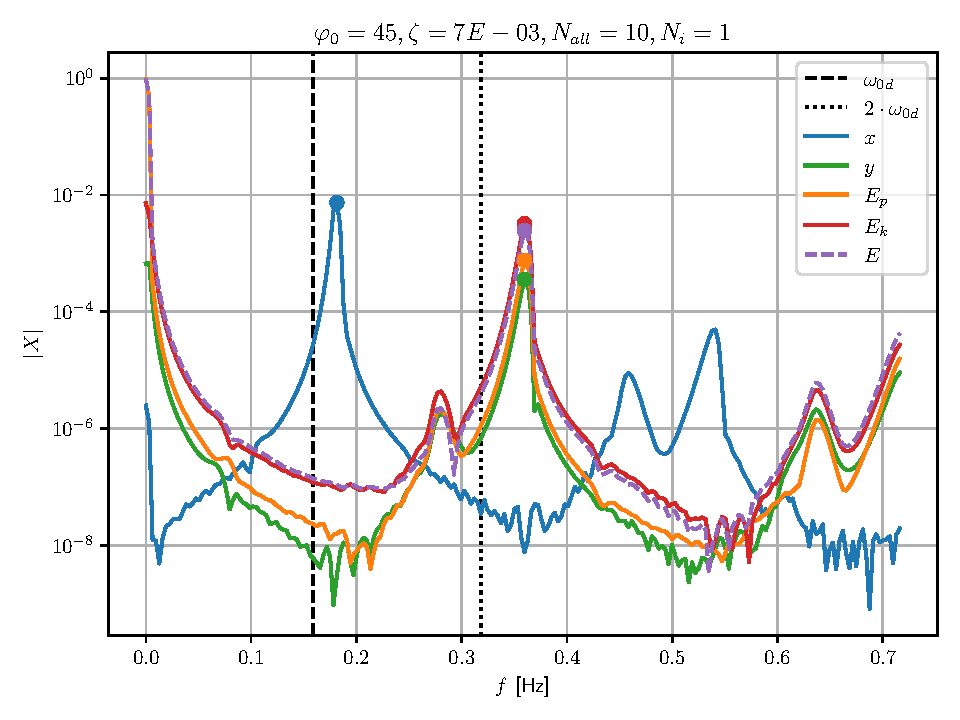
\includegraphics[width=\linewidth]{11.nal_slike/dinamika/fft_lastne_Ni1_phi45_N10.pdf}
            \caption{Amplitudni spekter v prvi masi}
        \end{subfigure}
        \begin{subfigure}{\linewidth}
            \centering
            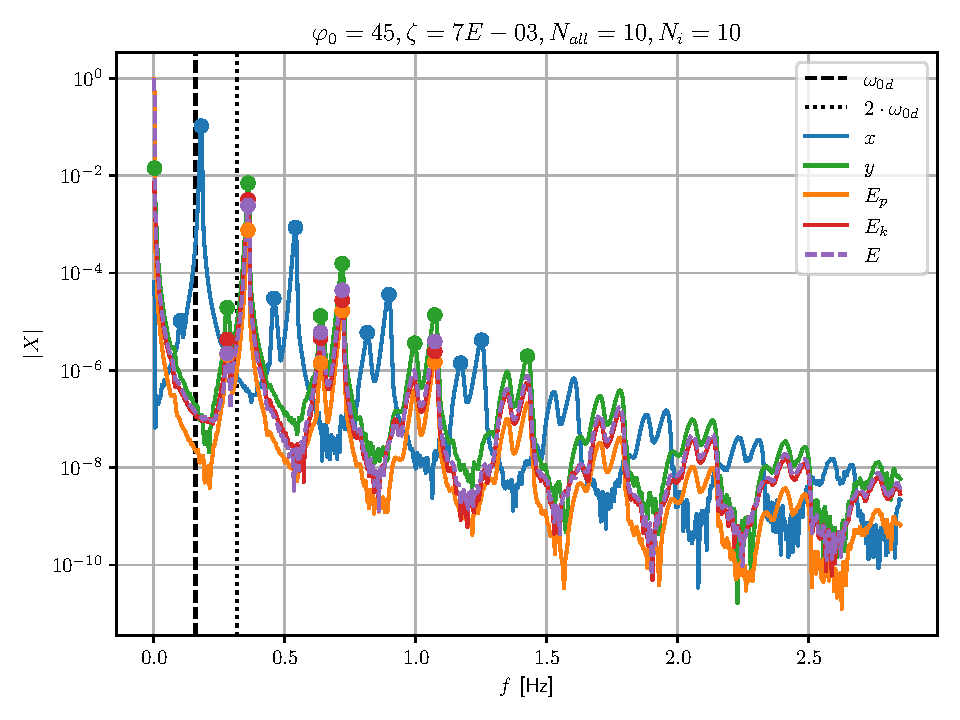
\includegraphics[width=\linewidth]{11.nal_slike/dinamika/fft_lastne_Ni10_phi45_N10.pdf}
            \caption{Amplitudni spekter v zadnji masi}
        \end{subfigure}
    \end{minipage}
    \begin{minipage}{0.45\textwidth}
        \centering
        \begin{subfigure}{\linewidth}
            \centering
            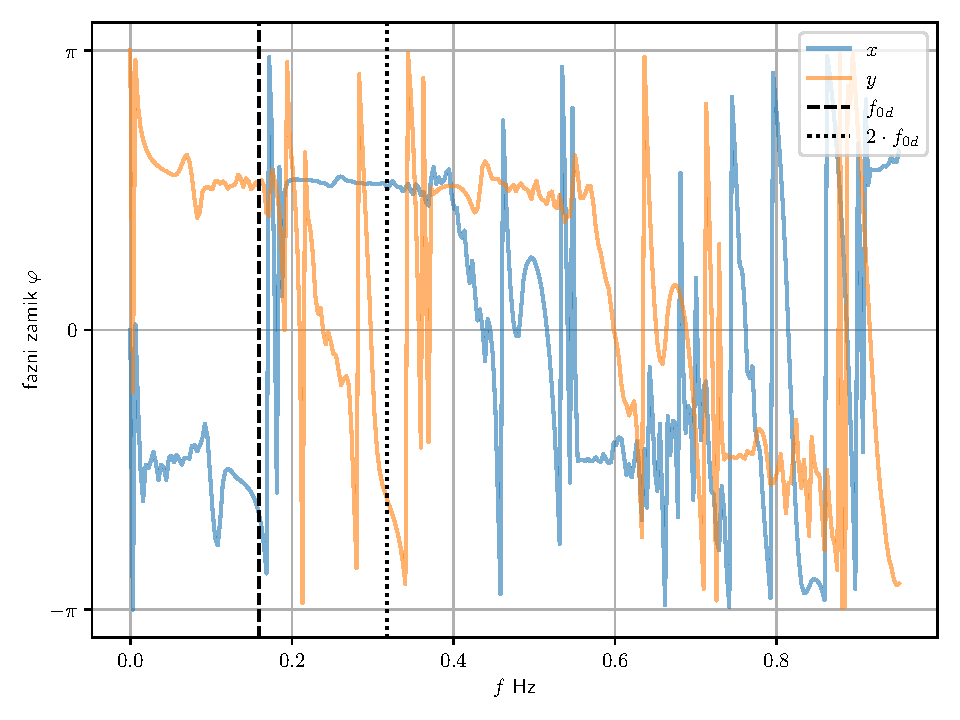
\includegraphics[width=\linewidth]{11.nal_slike/dinamika/fazni zamik_N10_phi45_N10.pdf}
            \caption{Fazni spekter v zadnji masi}
        \end{subfigure}
        \begin{subfigure}{\linewidth}
            \centering
            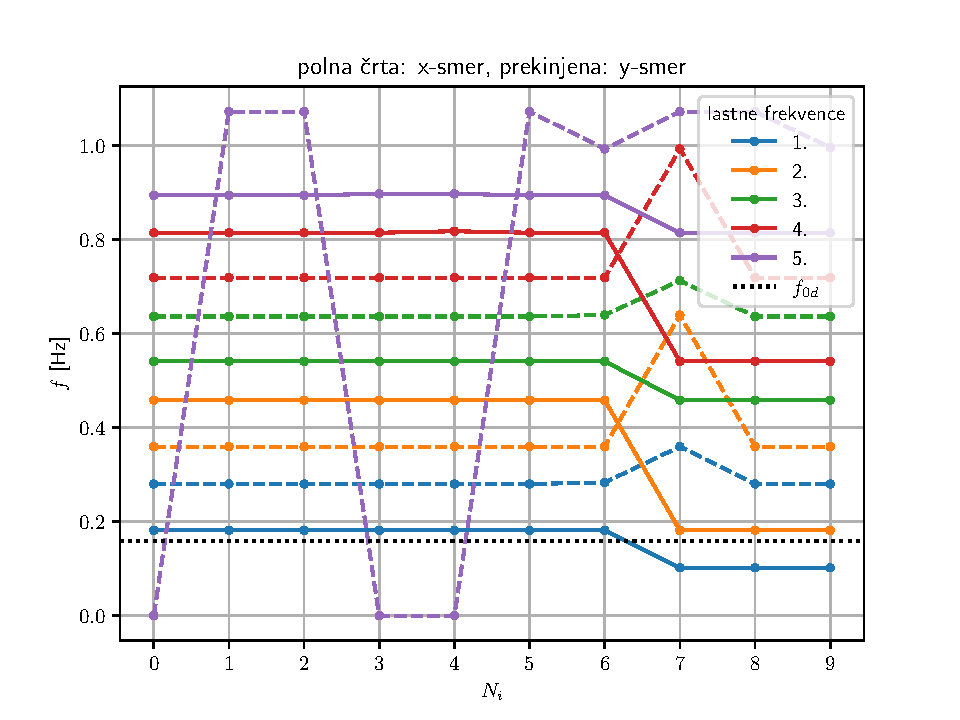
\includegraphics[width=\linewidth]{11.nal_slike/dinamika/vse_lastne_od_lege_phi45_N10.pdf}
            \caption{Lastne frekvence}
        \end{subfigure}
    \end{minipage}
    \caption{FFT pri diskretizaciji $N=10$ in ZP ravna vrv $\varphi_0=45^\circ$}
\end{figure}

\begin{figure}[H]
    \centering
    \begin{minipage}{0.45\textwidth}
        \centering
        \begin{subfigure}{\linewidth}
            \centering
            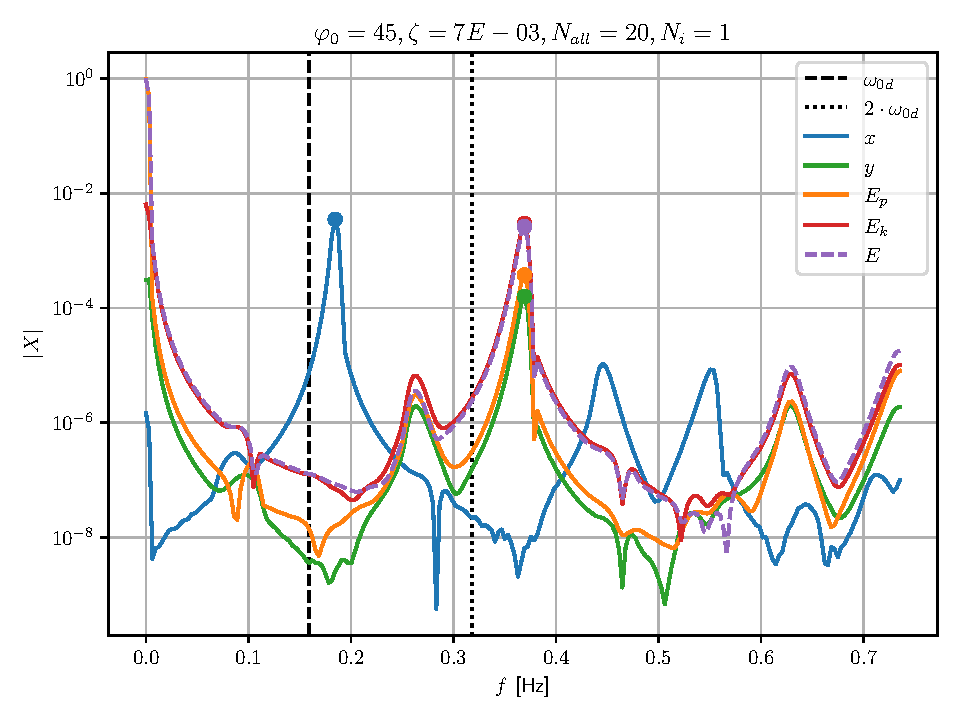
\includegraphics[width=\linewidth]{11.nal_slike/dinamika/fft_lastne_Ni1_phi45_N20.pdf}
            \caption{Amplitudni spekter v prvi masi}
        \end{subfigure}
        \begin{subfigure}{\linewidth}
            \centering
            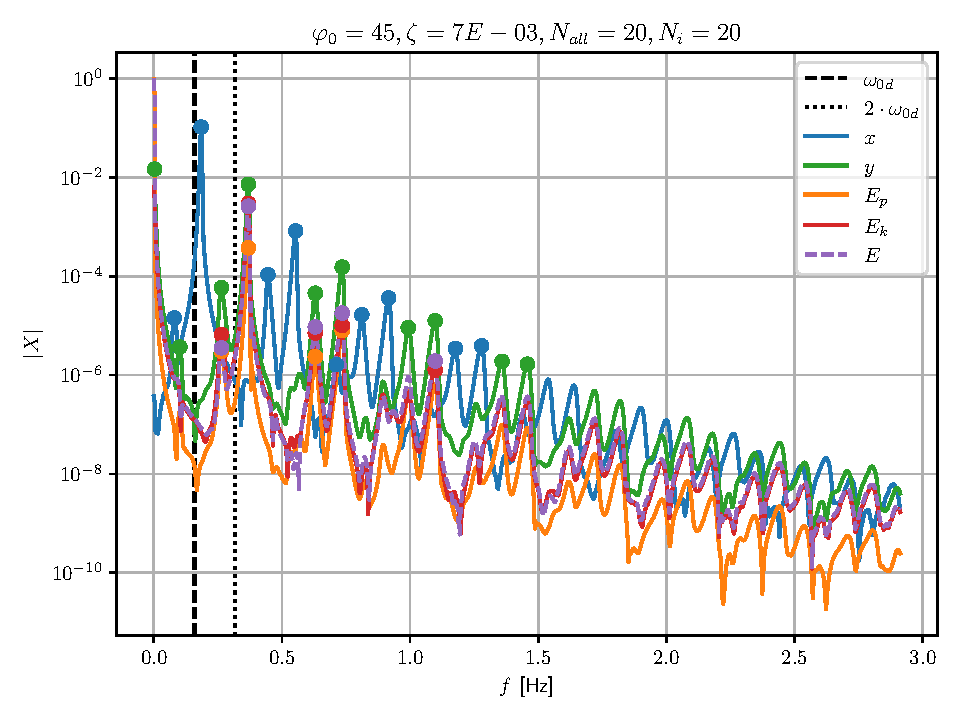
\includegraphics[width=\linewidth]{11.nal_slike/dinamika/fft_lastne_Ni20_phi45_N20.pdf}
            \caption{Amplitudni spekter v zadnji masi}
        \end{subfigure}
    \end{minipage}
    \begin{minipage}{0.45\textwidth}
        \centering
        \begin{subfigure}{\linewidth}
            \centering
            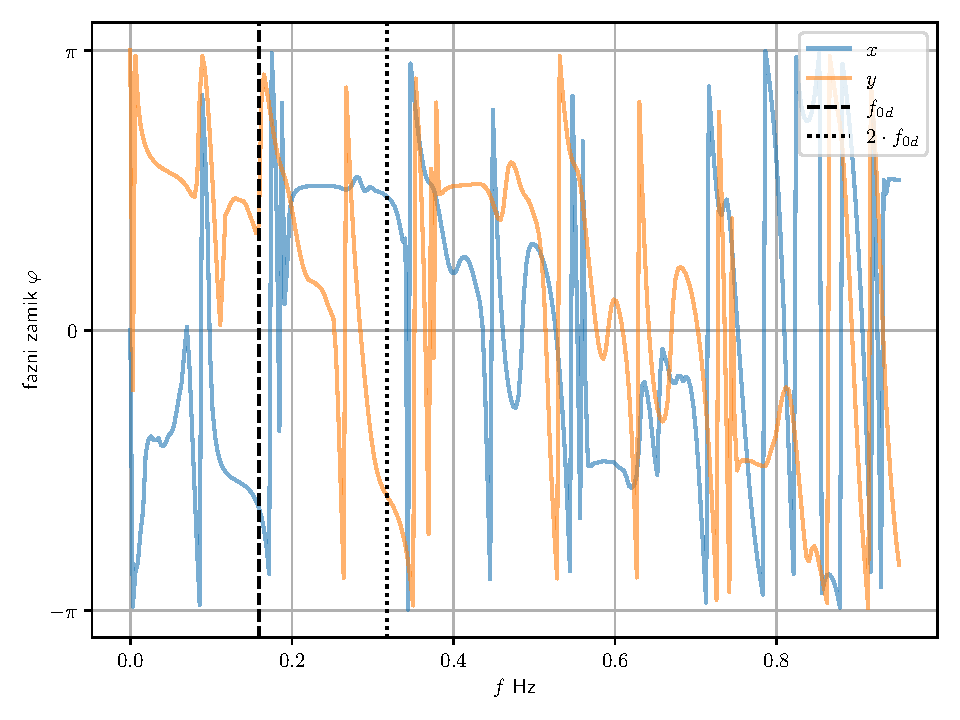
\includegraphics[width=\linewidth]{11.nal_slike/dinamika/fazni zamik_N20_phi45_N20.pdf}
            \caption{Fazni spekter v zadnji masi}
        \end{subfigure}
        \begin{subfigure}{\linewidth}
            \centering
            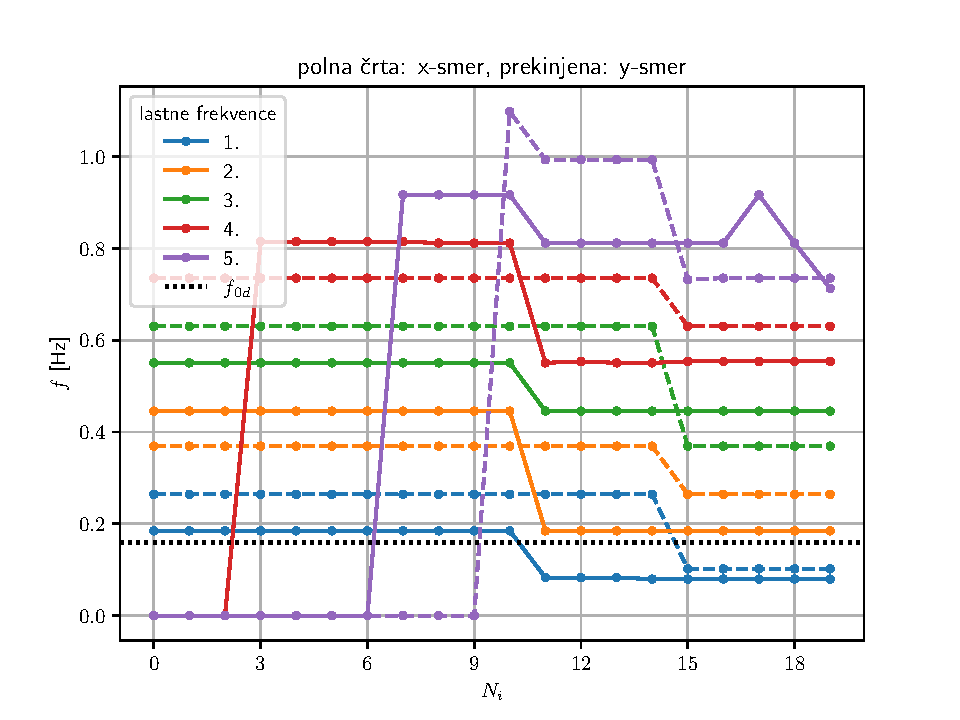
\includegraphics[width=\linewidth]{11.nal_slike/dinamika/vse_lastne_od_lege_phi45_N20.pdf}
            \caption{Lastne frekvence}
        \end{subfigure}
    \end{minipage}
    \caption{FFT pri diskretizaciji $N=20$ in ZP ravna vrv $\varphi_0=45^\circ$}
\end{figure}

\subsection{Odvisnost od začetnega kota}

Pri simulacijah sem povečeval začetni kot ravne vrvi $\varphi_0$ od 1$^\circ$ do 180$^\circ$. Ker se amplitudna spektra med prvo in zadnjo nihajočo maso ne razlikujeta bistveno, bom prikazoval vse na zadnji masi, kjer je zaradi večjih amplitud lažje določati vrhove. Opazim, da je lastna frekvenca (pričakovano) neodvisna od začetnega kota, le dovolj velik mora biti, da pride do nihanj, sicer pa vpliva na amplitudo!

Pri $\varphi_0=1^\circ$ zaradi majhne amplitude ne zaznamo lastne frekvence v y smeri zelo blizu izhodišča, sicer pa je v tem primeru še zelo malo šuma in so grafi precej lepi, kar se z večanjem kota pokvari.

Pri nadaljnjih primerih je ponovno težava šum na faznem spektru in frekvenčna ločljivost pri lastnih frekvencah, vendar je pri $\varphi_0=90^\circ$ vseeno opazno, da lastne frekvence niso več konstantne po vrvi, pri $\varphi_0=180^\circ$ pa je graf že premalo berljiv. Prav tako se je podrla značilnost, da je lastna frekvenca v y-smeri dvakratnik one v x-smeri.

Zanimivo je, da, kot sem že ugotovil v prejšnjem poglavju, je potek nihanja za $\varphi_0=180^\circ$ in $\varphi_0=-180^\circ$ ravno zrcalen. Isto se vidi tudi iz frekvenčne domene: amplitudna spektra sta enaka, fazni pa je le za y-smer zrcalen!

\begin{figure}[H]
    \centering
    \begin{minipage}{0.45\textwidth}
        \centering
        \begin{subfigure}{\linewidth}
            \centering
            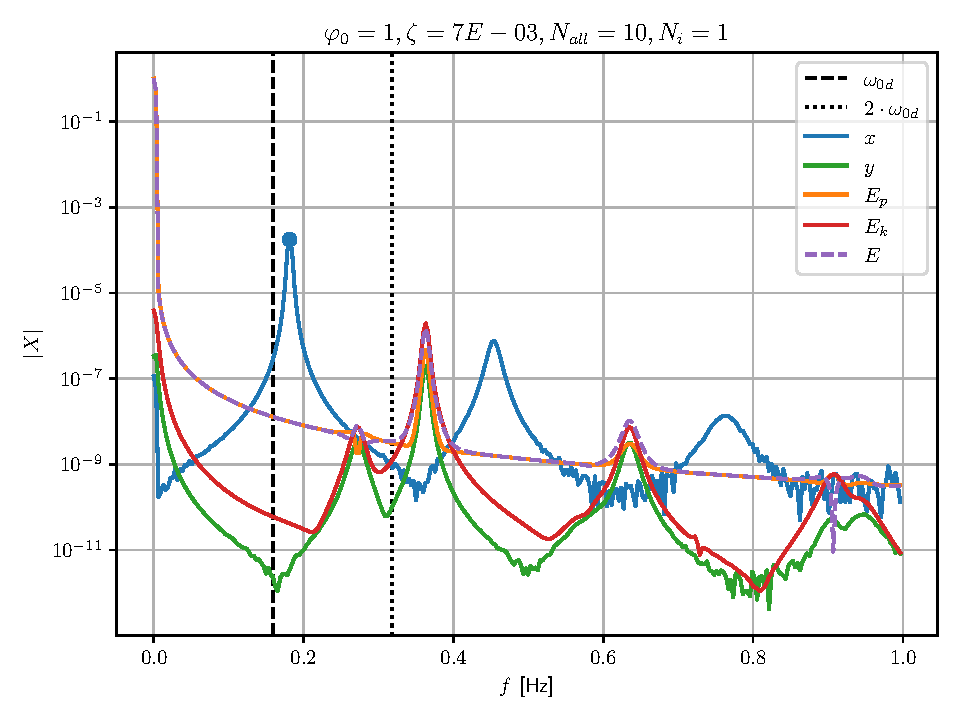
\includegraphics[width=\linewidth]{11.nal_slike/dinamika/phi/fft_lastne_Ni1_phi1_N10.pdf}
            \caption{Amplitudni spekter v prvi masi}
        \end{subfigure}
        \begin{subfigure}{\linewidth}
            \centering
            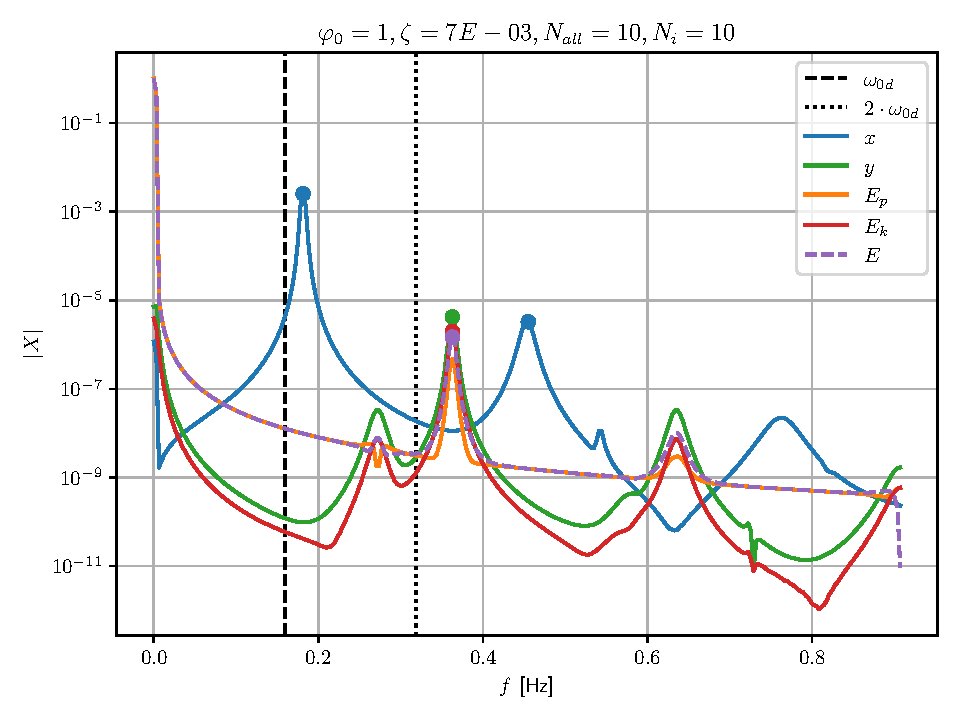
\includegraphics[width=\linewidth]{11.nal_slike/dinamika/phi/fft_lastne_Ni10_phi1_N10.pdf}
            \caption{Amplitudni spekter v zadnji masi}
        \end{subfigure}
    \end{minipage}
    \begin{minipage}{0.45\textwidth}
        \centering
        \begin{subfigure}{\linewidth}
            \centering
            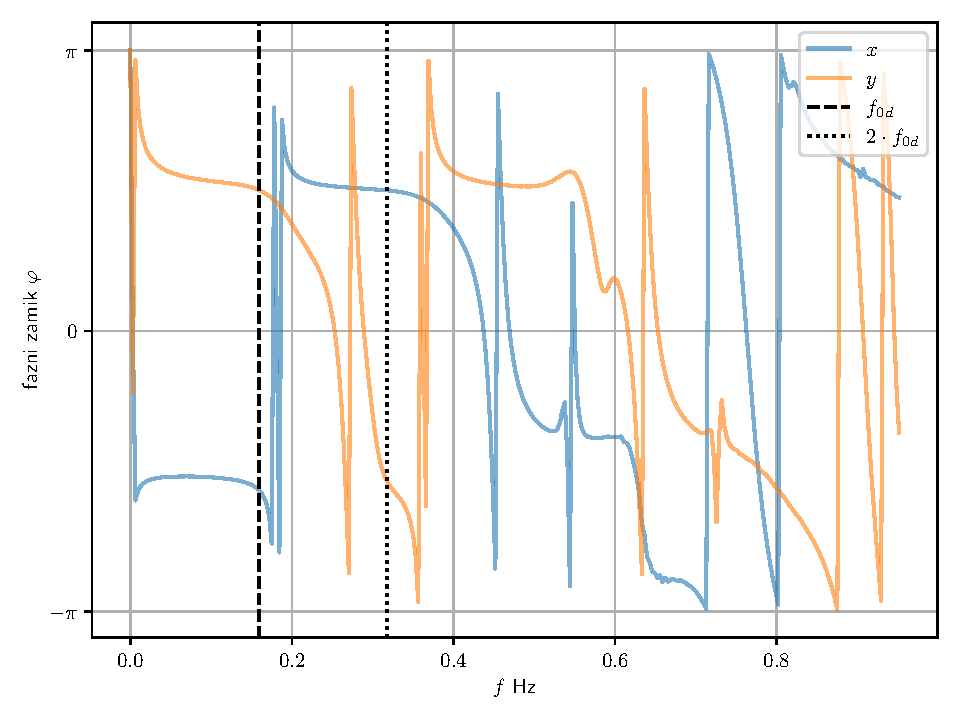
\includegraphics[width=\linewidth]{11.nal_slike/dinamika/phi/fazni zamik_N10_phi1_N10.pdf}
            \caption{Fazni spekter v zadnji masi}
        \end{subfigure}
        \begin{subfigure}{\linewidth}
            \centering
            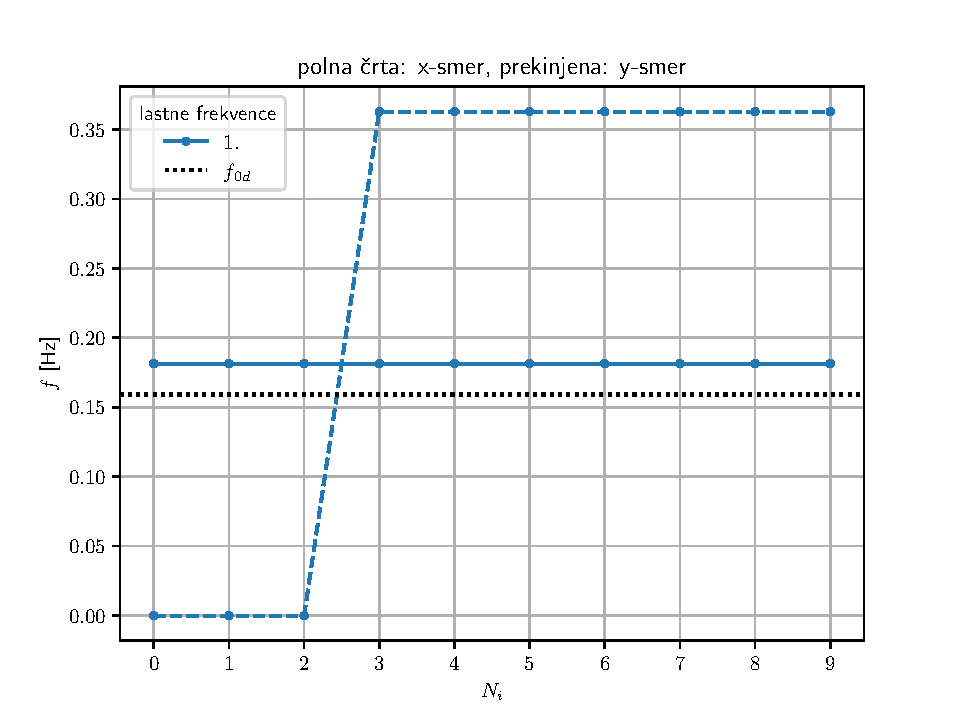
\includegraphics[width=\linewidth]{11.nal_slike/dinamika/phi/vse_lastne_od_lege_phi1_N10.pdf}
            \caption{Lastne frekvence}
        \end{subfigure}
    \end{minipage}
    \caption{FFT pri diskretizaciji $N=10$ in ZP ravna vrv $\varphi_0=1^\circ$}
\end{figure}

\begin{figure}[H]
    \centering
    \begin{minipage}{0.45\textwidth}
        \centering
        \begin{subfigure}{\linewidth}
            \centering
            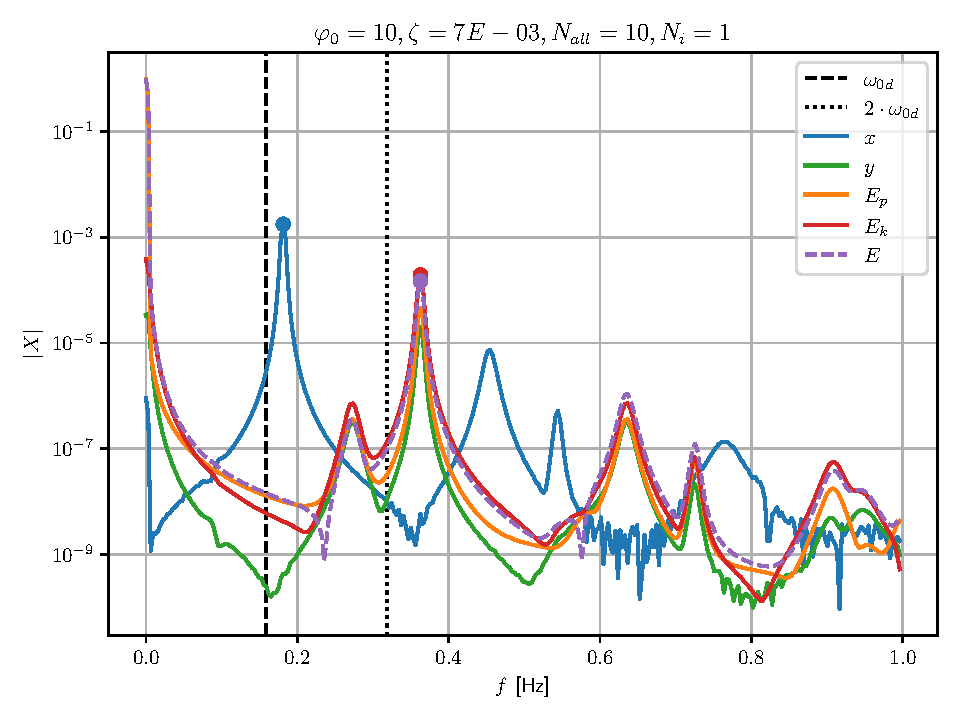
\includegraphics[width=\linewidth]{11.nal_slike/dinamika/phi/fft_lastne_Ni1_phi10_N10.pdf}
            \caption{Amplitudni spekter v prvi masi}
        \end{subfigure}
        \begin{subfigure}{\linewidth}
            \centering
            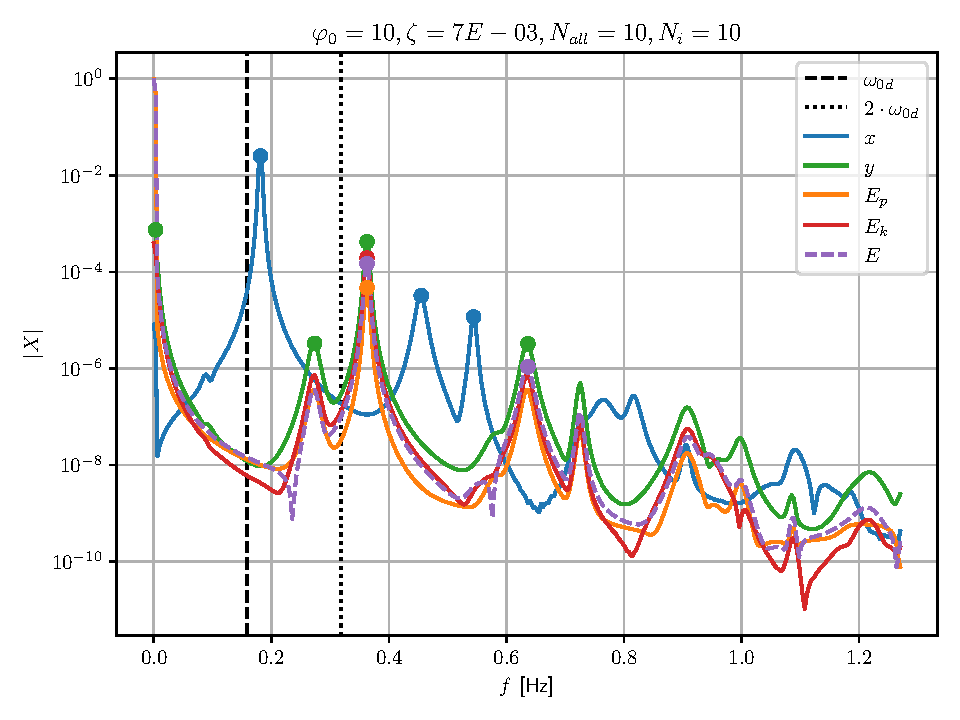
\includegraphics[width=\linewidth]{11.nal_slike/dinamika/phi/fft_lastne_Ni10_phi10_N10.pdf}
            \caption{Amplitudni spekter v zadnji masi}
        \end{subfigure}
    \end{minipage}
    \begin{minipage}{0.45\textwidth}
        \centering
        \begin{subfigure}{\linewidth}
            \centering
            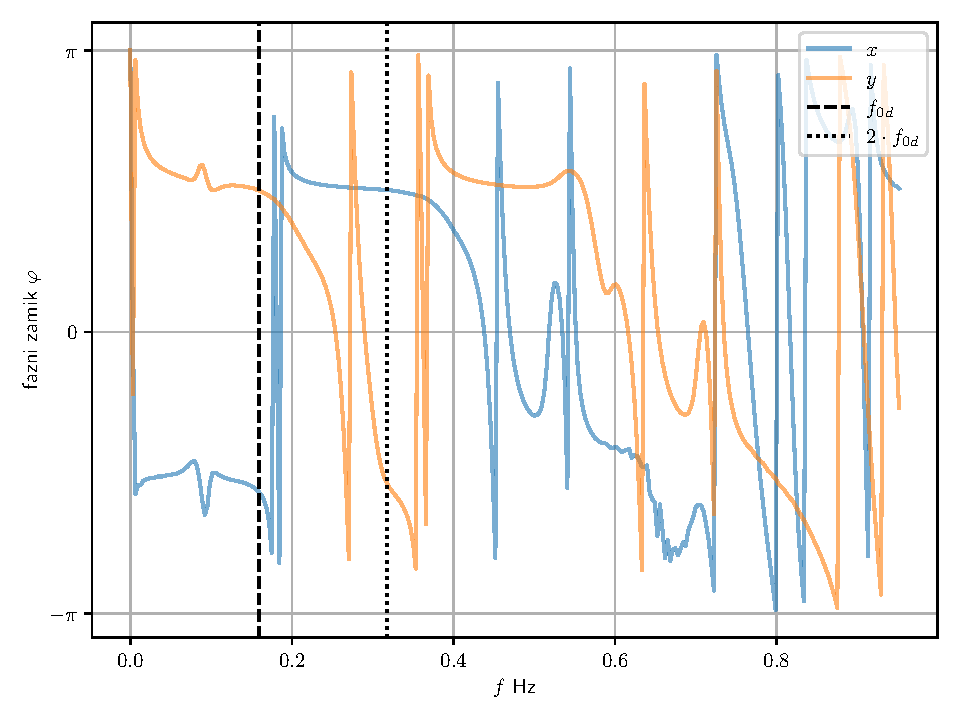
\includegraphics[width=\linewidth]{11.nal_slike/dinamika/phi/fazni zamik_N10_phi10_N10.pdf}
            \caption{Fazni spekter v zadnji masi}
        \end{subfigure}
        \begin{subfigure}{\linewidth}
            \centering
            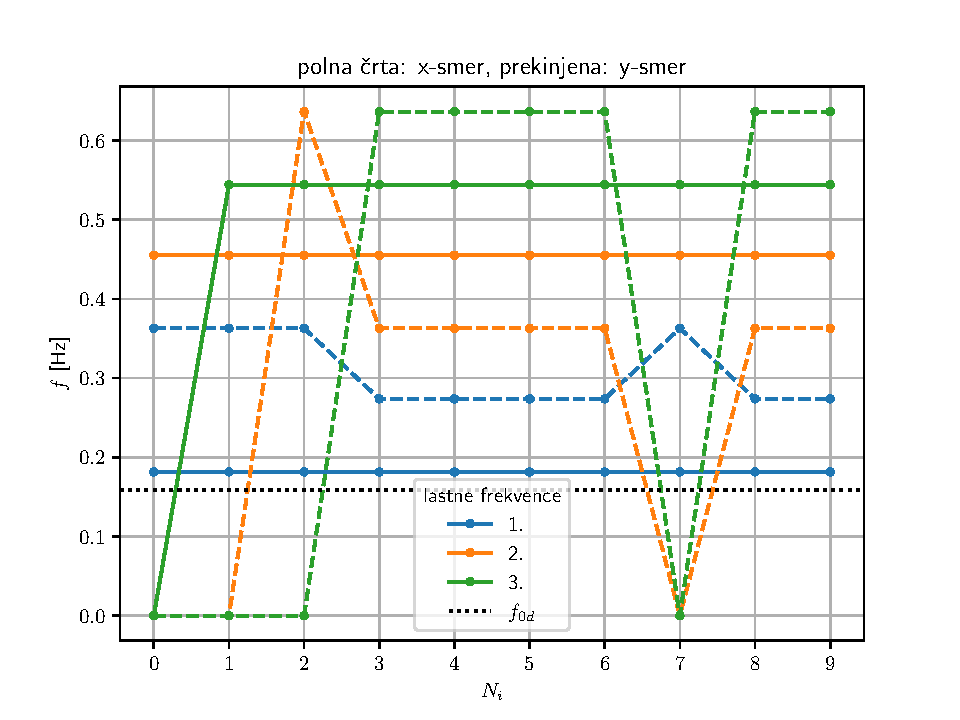
\includegraphics[width=\linewidth]{11.nal_slike/dinamika/phi/vse_lastne_od_lege_phi10_N10.pdf}
            \caption{Lastne frekvence}
        \end{subfigure}
    \end{minipage}
    \caption{FFT pri diskretizaciji $N=10$ in ZP ravna vrv $\varphi_0=10^\circ$}
\end{figure}

\begin{figure}[H]
    \centering
    \begin{subfigure}{0.49\textwidth}
        \centering
        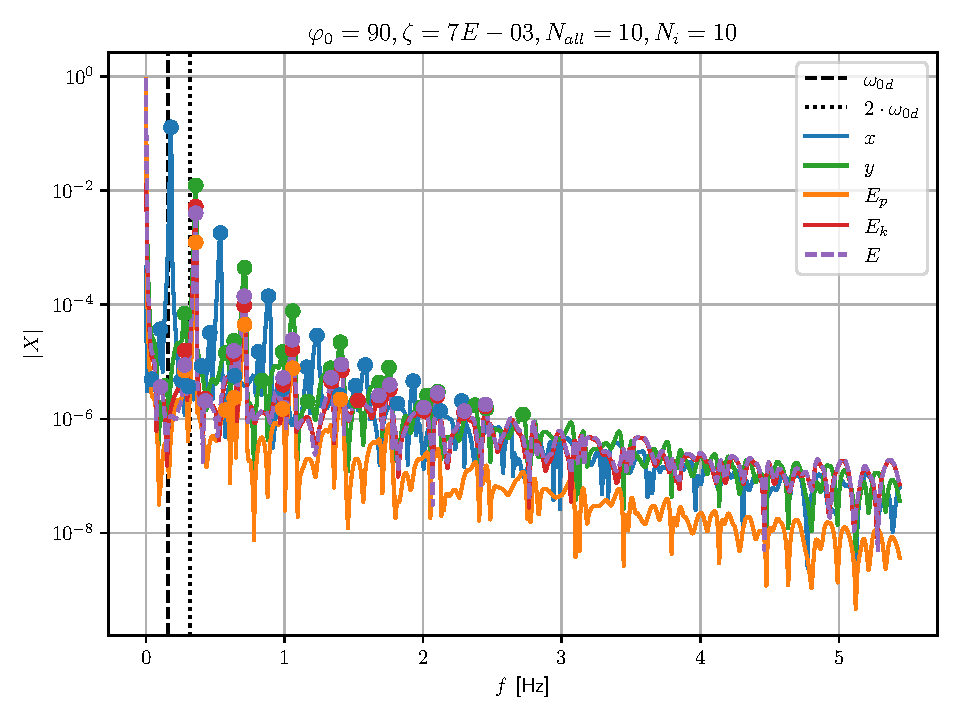
\includegraphics[width=\linewidth]{11.nal_slike/dinamika/phi/fft_lastne_Ni10_phi90_N10.pdf}
        \caption{Amplitudni spekter v zadnji masi}
    \end{subfigure}
    \begin{subfigure}{0.49\textwidth}
        \centering
        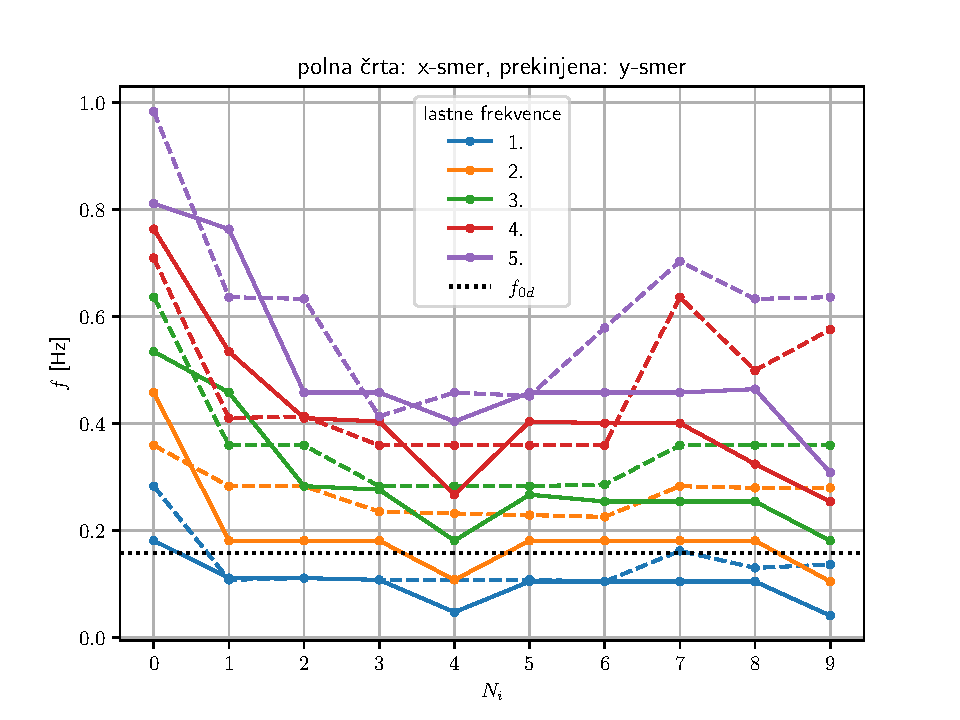
\includegraphics[width=\linewidth]{11.nal_slike/dinamika/phi/vse_lastne_od_lege_phi90_N10.pdf}
        \caption{Lastne frekvence}
    \end{subfigure}
    \caption{FFT pri diskretizaciji $N=10$ in ZP ravna vrv $\varphi_0=90^\circ$}
\end{figure}

\begin{figure}[H]
    \centering
    \begin{subfigure}{0.49\textwidth}
        \centering
        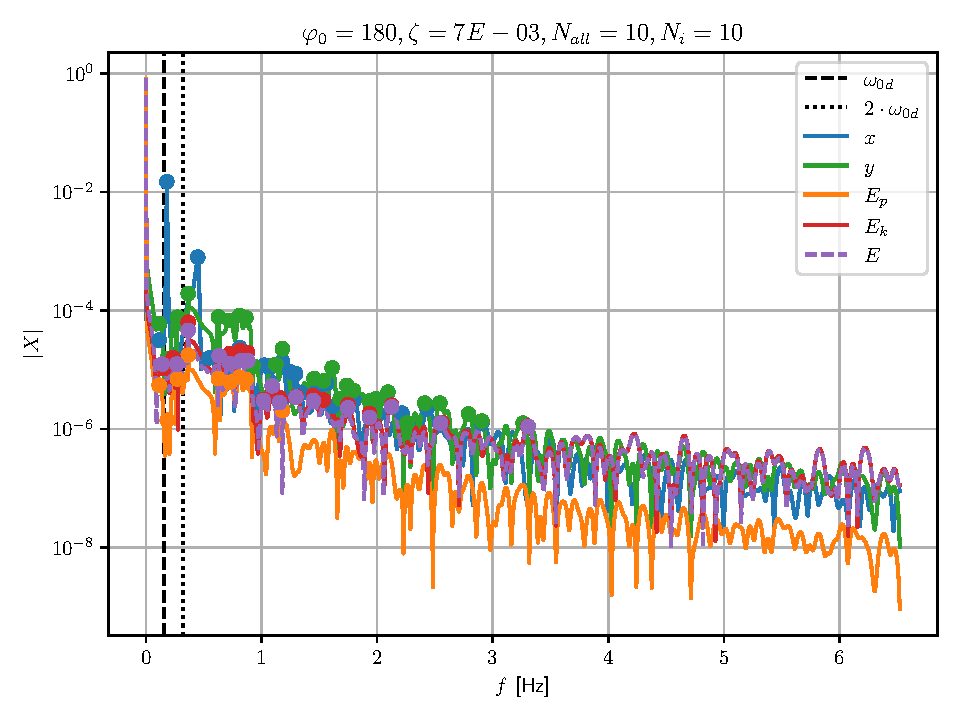
\includegraphics[width=\linewidth]{11.nal_slike/dinamika/phi/fft_lastne_Ni10_phi180_N10.pdf}
        \caption{Amplitudni spekter v zadnji masi}
    \end{subfigure}
    \begin{subfigure}{0.49\textwidth}
        \centering
        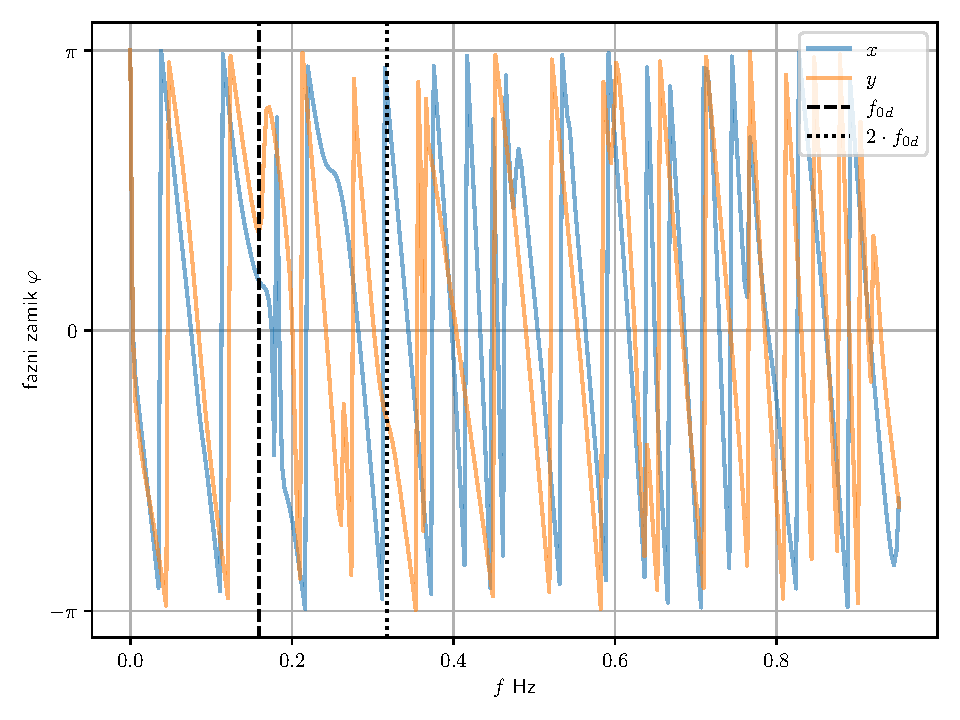
\includegraphics[width=\linewidth]{11.nal_slike/dinamika/phi/fazni zamik_N10_phi180_N10.pdf}
        \caption{Fazni spekter v zadnji masi}
    \end{subfigure}
    \caption{FFT pri diskretizaciji $N=10$ in ZP ravna vrv $\varphi_0=180^\circ$}
\end{figure}

\begin{figure}[H]
    \centering
    \begin{subfigure}{0.49\textwidth}
        \centering
        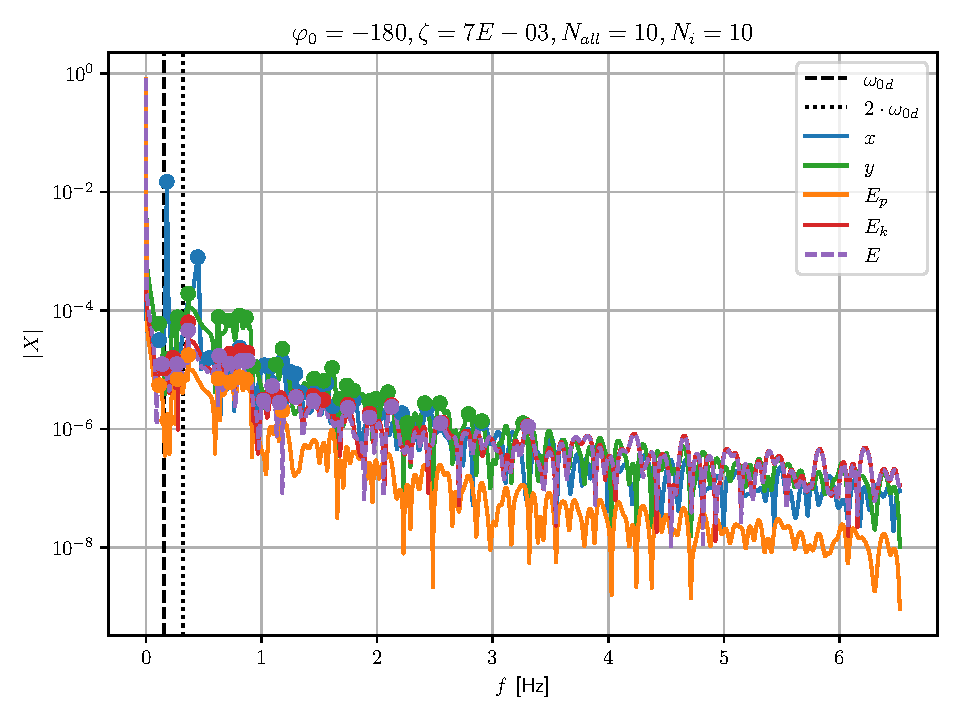
\includegraphics[width=\linewidth]{11.nal_slike/dinamika/phi/fft_lastne_Ni10_phi-180_N10.pdf}
        \caption{Amplitudni spekter v zadnji masi}
    \end{subfigure}
    \begin{subfigure}{0.49\textwidth}
        \centering
        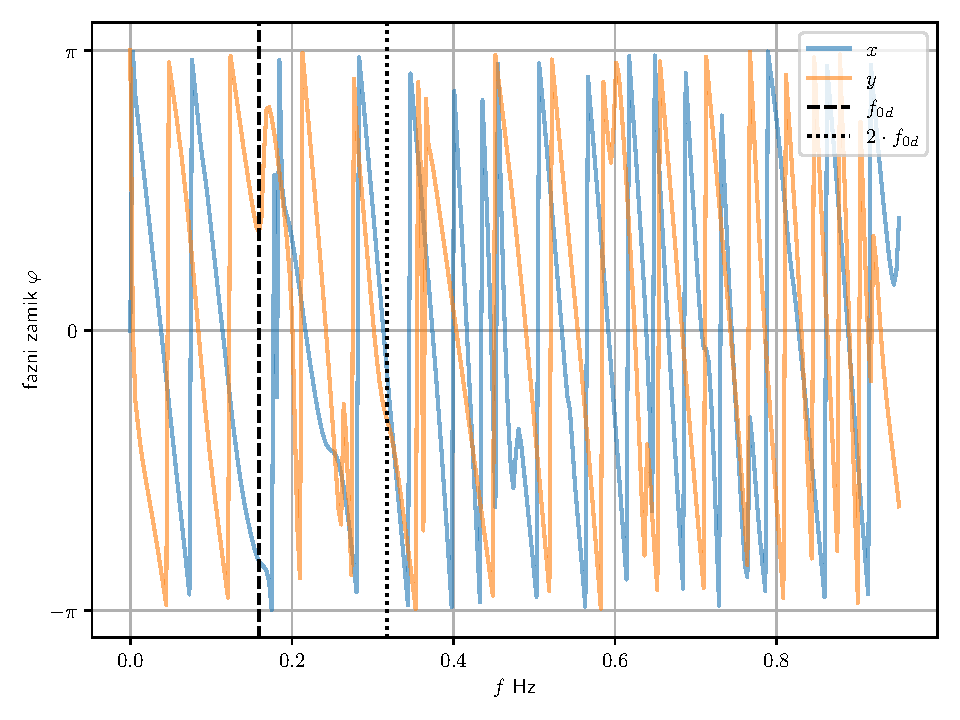
\includegraphics[width=\linewidth]{11.nal_slike/dinamika/phi/fazni zamik_N10_phi-180_N10.pdf}
        \caption{Lastne frekvence}
    \end{subfigure}
    \caption{FFT pri diskretizaciji $N=10$ in ZP ravna vrv $\varphi_0=-180^\circ$}
\end{figure}